\documentclass[titlepage]{article}
\usepackage[T1]{fontenc}
\usepackage{amsmath}
\usepackage{babel}
\usepackage{graphicx}


\graphicspath{{./images/}}

% widen margins
\usepackage[margin=1in]{geometry}

\author{
    Meisel, Carlos \\
  \and
  Juarez, Albert\\
  \and
    Quintero, Osvaldo\\
}
\title{Performance Analysis of the PT6A-114A Engine}
\begin{document}
  \maketitle

  \tableofcontents

  \vspace*{4cm}

    \section{Preface}

    Dear Dr.Cizmas,
    \vspace{0.5cm}

    I want to thank you for the hard work you have demanded of me in order to be a successful student in both of the courses that I took
    under your instructioning. Our office hours meeting, following the Fall 2021 AERO 351 Exam 2 test grades release, still resonates in my mind. 
    Up to that point, I had preformed poorly in the course, and it seemed as though I wasn't going to be able to pass the course. 
    As you may recall, it was my third attempt at the course, and I was in danger of violating the "3-peat" rule. After that meeting, with your advice
    I studied harder than I had ever studied before, and I was able to perform well on the final exam and pass the course. But the more 
    importantly that sucess continued and I went on to make the Dean's List the following semester (Spring 2022), a feat that I had never accomplished before.
    I took that same initative into my career aspirations securing two internships, one in the Summer 2022 at Arkisys, and another in Fall 2022 
    (current) with Loopback Analytics. Upon graduation, I will be joing Loopback Analytics as a Data/Machine Learning Engineer. While I 
    may be leaving aerospace engineering for software engineering, I want to credit you for work ethic and drive you have instilled in me.

    \vspace{0.5cm}

    Thank you for everything, 

    Carlos Meisel

    \vspace{1cm}

    Dear Dr.Cizmas,
    \vspace{0.5cm}

    I would like to take this time to thank you for all the knowledge you have given me. The way you pushed us in class made me become a better student and engineer. You have been the most influential person during my time in college. Upon graduation, I will be joining Los Alamos National Laboratory as an R \& D engineer. I will forever be grateful for the impact you have made on my life.

    \vspace{0.5cm}
    Thank you,

    Albert Juarez

    \vspace{1cm}


    Dr. Cizmas, 
    \vspace{0.5cm}

    I wanted to thank you for this past semester, you have been the one of the most interesting professors that I had the opportunity to study under. When I took Aero 351 with you, I considered it to be one of the most interesting classes that I had ever taken up to that point in my undergraduate career. Although I did not get an A in that course, I extremely enjoyed coming to class and listening to your lectures. Upon my graduation I will either be working in the private sector at Lockheed Martin or for the government at Los Alamos National Lab, my final decision is yet to be decided at this point. I hope to study under you in the future, until then, take care and hope life treats you well.

    \vspace{0.5cm}

    Sincerely,

    Osvaldo Quintero

    \vspace{5cm}

    \section{Engine Introduction}

    As per the Pratt and Whitney website, the PT6A-114 is a turboprop engine that is used in a variety of applications. 
    The PT6A class is the most popular engine in the world for its class and one of Pratt and Whitney's greatest success stories.
    The PT6A is used in a variety of applications, specifically for this project we will be looking at the PT6A-114A engine; which is 
    primarily used by the Cessna 208/208B Caravan I. 

    \section{Full Nominal Engine Cycle - Task 1}

    As stated earlier, the PT6A-114 engine is a Turboprop engine.
    A turboprop engine creates power from a shaft. Thrust is then produced from a combination of the propeller as well as the exhaust gas. The thrust produced from the propeller is far above the thrust provided by the exhaust gas. Given shaft horsepower, the efficiency of the compressor, and the inlet temperature of the turbine we find the specific thrust of the engine.

    Below is a list of given engine parameters:

    \begin{equation}
        \begin{aligned}
            \text{Shaft Horsepower, $SHP$} &= \text{600 hp} \\
            \text{Compressor Efficiency, $\eta_{comp}$} &= \text{0.90} \\
            \text{Turbine Inlet Temperature, $TIT$} &= \text{1410 K} \\
            \text{Compressor Ratio, $\pi_{c}$} &= \text{9.2} \\
            \text{Turbine Efficiency, $\eta_{turb}$} &= \text{0.94} \\
            \text{Combustor Efficiency, $\eta_{comb}$} &= \text{0.90} \\
            \text{Free Turbine Efficiency, $\eta_{PT}$} &= \text{0.94} \\
            \text{Nozzle Efficiency, $\phi_{nozzle}$} &= \text{0.98} \\
            \text{Propeller Efficiency, $\eta_{prop}$} &= \text{0.8} \\
            \text{Diffuser Efficiency, $\eta_{d}$} &= \text{0.99} \\
        \end{aligned}
    \end{equation}

    \subsection{Stage a}

    We begin at static conditions, specifically here we are calculating the static conditions at take-off. Since we are at take-off conditions, one can assume sea level atmospheric conditions.

    \begin{equation}
        \begin{aligned}
            \text{Static Pressure, $p_{a}$} &= 101.325 \text{ kPa} \\
            \text{Static Temperature, $T_{a}$} &= 288.16 \text{ K} \\
        \end{aligned}
    \end{equation}

    By knowing the Temperature $T_{a}$ we are able to calculate enthalpy from the air gas tables:

    \begin{equation}
        h_{a}(T_{a})_{Tables} = 288.299988 \frac{kJ}{kg}
    \end{equation}

    And for entropy:

    \begin{equation}
        s_{a_{p=1 bar}}(T_{a})_{Tables} = 6.6570201 \frac{kJ}{kg K}
    \end{equation}

    After reading from the tables for entropy, we will need to normalize to the static pressure of $p_{a}$.

    \begin{equation}
        s_{a} = s_{a_{p=1 bar}}(T_{a}) - R \ln \left( \frac{p_{a}}{1 \text{ bar}} \right)
    \end{equation}

    \subsection{Stage 0a}
    In this stage we going to assume that stage 0a is equivalent to stage a. 

    \begin{equation}
        \begin{aligned}
            \text{$p_{0a}$} &= 101.325 \text{ kPa} \\
            \text{$T_{0a}$} &= 288.16 \text{ K} \\
            \text{$h_{0a}$} &= 288.299988 \frac{kJ}{kg} \\
            \text{$s_{0a}$} &= 6.6570201 \frac{kJ}{kg K} \\
        \end{aligned}
    \end{equation}

    \subsection{Stage 01}

    Here in this stage, we take into account the Diffuser. 

    \begin{equation} 
        p_{01} = p_{0a} \eta_{d}
    \end{equation}

    \begin{equation}
        T_{01} = T_{0a} 
    \end{equation}

    \begin{equation}
        h_{01}(T_{01})_{Tables} = 288.299988 \frac{kJ}{kg}
    \end{equation}

    \begin{equation}
        s_{01_{p= 1 bar}}(T_{01})_{Tables} = 6.6570201 \frac{kJ}{kg K}
    \end{equation}

    \begin{equation}
        s_{01} = s_{01_{p=1 bar}}(T_{01}) - R \ln \left( \frac{p_{01}}{1 \text{ bar}} \right)
    \end{equation}

    \subsection{Stage 02i}

    Here we are calculating the isentropic conditions of the compressor, stage 02i. At this point, we say that:

    \begin{equation}
        s_{02i} = s_{01}
    \end{equation}

    Calculating the pressure, we use the pressure ratio of the compressor:

    \begin{equation}
        p_{02i} = p_{01} \pi_{c}
    \end{equation}

    Recall, we need to normalize the entropy to 1 bar pressure to be used for the tables:

    \begin{equation}
        s_{02i_{p=1 bar}} =  s_{02i}+ R \ln \left( \frac{p_{02i}}{1 \text{ bar}} \right)
    \end{equation}

    We can use the entropy found, to use the H method, to find enthalpy:

    \begin{equation}
        h_{02i}(s_{02i_{p=1 bar}})_{Tables} =  543.819 \frac{kJ}{kg}
    \end{equation}

    We can now calculate the ideal work of the compressor:

    \begin{equation}
        w_{02i} = h_{02i} - h_{01}
    \end{equation}


    \subsection{Stage 02}

    The pressure at Stage 02 is the same as the pressure at Stage 02i. This allows for us to move forward through the engine cycle.

    \begin{equation}
        p_{02} = p_{02i}
    \end{equation}

    \begin{center}
        \begin{tabular}{|c|}
            \hline
            $p_{02}$ \\
            \hline
            9.228681 \text{ bar} \\
            \hline
        \end{tabular}
    \end{center}

    Using the ideal work of the compressor, we can calculate the actual work of the compressor:

    \begin{equation}
        w_{02} = \frac{ w_{02i}}{ \eta_{comp}}
    \end{equation}

    \begin{center}
        \begin{tabular}{|c|}
            \hline
            $w_{02}$ \\
            \hline
            283.91025 \text{ kJ/kg} \\
            \hline
        \end{tabular}
    \end{center}

    This will allow for us to easily calculate the enthalpy.

    \begin{equation}
        h_{02} = h_{01} + w_{02}
    \end{equation}

    This enthalpy can now be used for the S method, to find entropy:

    \begin{equation}
        s_{02_{p=1 bar}}(h_{02})_{Tables} =  6.7113694 \frac{kJ}{kg K}
    \end{equation}

    Finally we normalize the entropy:

    \begin{equation}
        s_{02} = s_{02_{p=1 bar}} - R \ln \left( \frac{p_{02}}{1 \text{ bar}} \right)
    \end{equation}

    \subsection{Stage 03}

    We were given a pressure drop in the combustor of $3 \%$. Resulting in the following pressure:

    \begin{equation}
        p_{03} = p_{02} \left( 1 - \frac{3}{100} \right)
    \end{equation}

    \begin{center}
        \begin{tabular}{|c|}
            \hline
            $p_{03}$ \\
            \hline
            8.95182057 \text{ bar} \\
            \hline
        \end{tabular}
    \end{center}

    We are also given a $T_{03}$ of 1410 K.

    \begin{equation}
        h_{03_{air}}(T_{03})_{Air Tables} = h_{03_{air}}
    \end{equation} 

    \begin{equation} 
        h_{03_{\lambda=1}}(T_{03})_{Stoich  Tables} = h_{03_{\lambda=1}}
    \end{equation}

    We then use the two above equations to calculate excess air:

    \begin{equation}
        \lambda = \frac{h_{03_{\lambda=1}} (1+minL) - \eta_{comb}LHV -h_{03_{air}}minL}{minL (h_{02}-h_{03_{air}})}
    \end{equation}

    Recall:

    \begin{equation}
        \begin{aligned}
            \text{$LHV$} &=  43.5 \frac{kJ}{kg} \\
            \text{$minL$} &=  14.66 \\
        \end{aligned}
    \end{equation}

    \begin{center}
        \begin{tabular}{|c|}
            \hline
            $\lambda$ \\
            \hline
            2.8537672 \\
            \hline
        \end{tabular}
    \end{center}

    We can now calculate our weighting functions:

    \begin{equation}
        r = \frac{1 + minL}{1 + \lambda minL}
    \end{equation}

    \begin{equation}
        q = \frac{(\lambda -1)minL}{1+\lambda minL}
    \end{equation}

    With the weighting functions, we can now calculate the enthalpy of the mixture:

    \begin{equation}
        h_{03} = r h_{03_{\lambda=1}} + q h_{03_{air}}
    \end{equation}

    Similar to how we calculated the enthalpies from the table, we will now calculate the entropy of the mixture:

    \begin{equation}
        s_{03_{air, p= 1 bar}}(T_{03})_{Air Tables} = s_{03_{air, p=1 bar}}
    \end{equation} 

    \begin{equation}
        s_{03_{\lambda=1, p= 1 bar}}(T_{03})_{Stoich  Tables} = s_{03_{\lambda=1, p = 1 bar}}
    \end{equation}

    \begin{equation}
        s_{03_{p=1 \lambda}} = r s_{03_{\lambda=1, p=1 bar}} + q s_{03_{air, p=1 bar}}
    \end{equation}

    \subsection{Stage 04i}
    The entropy of stage 04i is the same as the entropy of stage 03. This allows for us to move forward through the engine cycle.

    \begin{equation}
        s_{04i} = s_{03}
    \end{equation}

    We make use of:

    \begin{equation}
        \mathcal{P}_{C} = \mathcal{P}_{T} 
    \end{equation}

    Which can be simplified to:

    \begin{equation}
        \dot{m}_{g}w_{T} = \dot{m}_{a}w_{C}
    \end{equation}

    \begin{equation}
        w_{T}= w_{C} \left( \frac{1}{1+ \frac{1}{\lambda minL}}\right)
    \end{equation}

    \begin{center}
        \begin{tabular}{|c|}
            \hline
            $w_{T}$ \\
            \hline
            277.2824 \text{ kJ/kg} \\
            \hline
        \end{tabular}
    \end{center}


    This will allow for us to calculate the ideal work of the turbine:

    \begin{equation}
        w_{T_{i}} = \frac{w_{T}}{\eta_{T}}
    \end{equation}

    We will use the ideal work of the turbine to calculate the enthalpy of stage 04i:

    \begin{equation}
        h_{04i} = h_{03} - w_{T_{i}}
    \end{equation}

    From here we will use the enthalpy $h_{04i}$ to calculate the Temperature of stage 04i. To do so, one must iterate, such that the following
    equation is satsified:

    \begin{equation}
        f(T) = h_{04i} - r h_{04i_{\lambda=1}}(T) - q h_{04i_{air}}(T) = 0
    \end{equation}

    Our group developed an iteration algorithm \verb|Iterate_temp_h| to solve for the temperature. The algorithm is as follows:

    \begin{center}
        $i = 1$ \\
        $h_{air} = h_{input}$ \\
        $T_{air_{i=1}}(h_{input})_{Air Tables} = T_{a_{i=1}}$ \\
        $h_{\lambda= 1_{i=1}}(T_{a_{i=1}})_{Stoich Tables} = h_{\lambda=1_{i=1}}$ \\

        \vspace*{0.5cm}

        $i=2$ \\
        $h_{\lambda=1_{i=2}} = h_{input}$ \\
        $T_{\lambda=1_{i=2}}(h_{input})_{Stoich Tables} = T_{\lambda=1_{i=2}}$ \\
        $h_{air_{i=2}}(T_{\lambda=1_{i=2}})_{Air Tables} = h_{air_{i=2}}$ \\

        \vspace*{0.5cm}

        $f(T)_{1} = h_{input} - r h_{\lambda=1_{i=1}} - q h_{air_{i=1}}$ \\
        $f(T)_{2} = h_{input} - r h_{\lambda=1_{i=2}} - q h_{air_{i=2}}$ \\

        \vspace*{0.5cm}

        $T = \frac{T_{air_{i=1}} * f(T)_{2} - T_{\lambda=1_{i=2}} * f(T)_{1}}{f(T)_{2} - f(T)_{1}}$ \\
    \end{center}

    After the \verb|Iterate_temp_h(h04i, r, q)| algorithm is ran, we now have our temperature $T_{04i}$. We can now begin out 
    entropy calculation.
    
    \begin{equation}
        s_{04i_{air, p= 1 bar}}(T_{04i})_{Air Tables} = s_{04i_{air, p=1 bar}}
    \end{equation} 

    \begin{equation}
        s_{04i_{\lambda=1, p= 1 bar}}(T_{04i})_{Stoich  Tables} = s_{04i_{\lambda=1, p = 1 bar}}
    \end{equation}

    \begin{equation}
        s_{04i_{p=1 \lambda}} = r s_{04i_{\lambda=1, p=1 bar}} + q s_{04i_{air, p=1 bar}}
    \end{equation}

    \begin{equation}
        s_{04i_{\lambda}} = s_{04i_{p=1 \lambda}} - R \ln \left( \frac{p_{04i}}{1 bar} \right)
    \end{equation}

    We can manipulate the above equation for pressure:

    \begin{equation}
        p_{04i} = e^{- \frac{s_{04i_{\lambda}} - s_{04i_{p=1 \lambda}}}{R}}
    \end{equation}

    \subsection{Stage 04}

    Moving from stage 04i to stage 04, we can assume no pressure change meaning:

    \begin{equation}
        p_{04} = p_{04i}
    \end{equation}

    We can calculate the enthalpy of stage 04 using the work of the turbine:

    \begin{equation}
        h_{04} = h_{03} - w_{T}
    \end{equation}

    From here we are to calculate the temperature by the iterations algorithm again:

    \begin{center}
        \verb|Iterate_temp_h(h04, r, q)| = $T_{04}$
    \end{center}

    We can use the temperature to calculate the entropy of stage 04:

    \begin{equation}
        s_{04_{air, p= 1 bar}}(T_{04})_{Air Tables} = s_{04_{air, p=1 bar}}
    \end{equation}

    \begin{equation}
        s_{04_{\lambda=1, p= 1 bar}}(T_{04})_{Stoich  Tables} = s_{04_{\lambda=1, p = 1 bar}}
    \end{equation}

    \begin{equation}
        s_{04_{p=1 \lambda}} = r s_{04_{\lambda=1, p=1 bar}} + q s_{04_{air, p=1 bar}}
    \end{equation}

    Finally we can calculate the entropy of stage 04, by normalizing the pressure:

    \begin{equation}
        s_{04_{\lambda}} = s_{04_{p=1 \lambda}} - R \ln \left( \frac{p_{04}}{1 bar} \right)
    \end{equation}

    \subsection{Stage 04.5i}

    One can assume that the transition from stage 04 to stage 04.5i is isentropic. This means that the entropy of stage 04.5i is equal to the entropy of stage 04:

    \begin{equation}
        s_{04.5i_{\lambda}} = s_{04_{\lambda}}
    \end{equation}

    The specific work of the of the free turbine is:

    \begin{equation}
        w_{PT} = \frac{SHP}{\dot{m}_{g}} = \frac{SHP}{\dot{m}_{a} (1 +f)}
    \end{equation}

    Which can be simplified as:

    \begin{equation}
        w_{PT} = \frac{SHP}{\dot{m}_{a} \left(1 + \frac{1}{\lambda minL}\right)}
    \end{equation}

    \begin{center}
        \begin{tabular}{|c|}
            \hline
            $w_{PT}$ \\
            \hline
            262.83965 kJ/kg \\
            \hline
        \end{tabular}
    \end{center}

    Now we can calculate the ideal work of the free turbine, by making use of its efficiency:

    \begin{equation}
        w_{PT_{i}} = \frac{w_{PT}}{\eta_{PT}}
    \end{equation}

    The enthalpy of stage 04.5i is:

    \begin{equation}
        h_{04.5i} = h_{04} - w_{PT_{i}}
    \end{equation}

    We can now calculate the temperature of stage 04.5i by using the iterations algorithm:

    \begin{center}
        \verb|Iterate_temp_h(h04.5i, r, q)| = $T_{04.5i}$
    \end{center}

    We can now calculate the entropy of stage 04.5i:

    \begin{equation}
        s_{04.5i_{air, p= 1 bar}}(T_{04.5i})_{Air Tables} = s_{04.5i_{air, p=1 bar}}
    \end{equation}

    \begin{equation}
        s_{04.5i_{\lambda=1, p= 1 bar}}(T_{04.5i})_{Stoich  Tables} = s_{04.5i_{\lambda=1, p = 1 bar}}
    \end{equation}

    \begin{equation}
        s_{04.5i_{p=1 \lambda}} = r s_{04.5i_{\lambda=1, p=1 bar}} + q s_{04.5i_{air, p=1 bar}}
    \end{equation}

    We can use this to calculate pressure:

    \begin{equation}
        p_{04.5i} = e^{ - \frac{s_{04.5i_{\lambda}} - s_{04.5i_{p=1 \lambda}}}{R}}
    \end{equation}

    \begin{center}
        \begin{tabular}{|c|}
            \hline
            $p_{04.5i}$ \\
            \hline
            1.6164346 bar \\
            \hline
        \end{tabular}
    \end{center}

    \subsection{Stage 04.5}

    The pressure at stage 04.5 is equal to the pressure at stage 04.5i:

    \begin{equation}
        p_{04.5} = p_{04.5i}
    \end{equation}

    The enthalpy of stage 04.5 is:

    \begin{equation}
        h_{04.5} = h_{04} - w_{PT}
    \end{equation}

    We will use the iterations algorithm to calculate the temperature of stage 04.5:

    \begin{center}
        \verb|Iterate_temp_h(h04.5, r, q)| = $T_{04.5}$
    \end{center}

    We can now calculate the entropy of stage 04.5:

    \begin{equation}
        s_{04.5_{air, p= 1 bar}}(T_{04.5})_{Air Tables} = s_{04.5_{air, p=1 bar}}
    \end{equation}

    \begin{equation}
        s_{04.5_{\lambda=1, p= 1 bar}}(T_{04.5})_{Stoich  Tables} = s_{04.5_{\lambda=1, p = 1 bar}}
    \end{equation}

    \begin{equation}
        s_{04.5_{p=1 \lambda}} = r s_{04.5_{\lambda=1, p=1 bar}} + q s_{04.5_{air, p=1 bar}}
    \end{equation}

    Normalize entropy by pressure:

    \begin{equation}
        s_{04.5_{\lambda}} = s_{04.5_{p=1 \lambda}} - R \ln \left( \frac{p_{04.5}}{1 bar} \right)
    \end{equation}


    \subsection{Stage 5i}
    The process from Stage 04.5 to Stage 5i is isentropic. This means that the entropy of stage 5i is equal to the entropy of stage 04.5:

    \begin{equation}
        s_{05i_{\lambda}} = s_{04.5_{\lambda}}
    \end{equation}

    And the pressure of stage 5i goes to atmospheric pressure:

    \begin{equation}
        p_{05i} = p_{a} = p_{01}
    \end{equation}

    Having determined the entropy of stage 5i and the pressure of stage 5i, we must now determine the temperature of stage 5i. We will use the iterations algorithm to calculate the temperature of stage 5i:
    The iterative process \verb|Iterate_temp_ps| is similar to \verb|Iterate_temp_h| algorithm however it solves:

    \begin{equation}
        f(T) = s_{5_{i}} - q s_{5_{i_{air}}}(T) - r s_{5_{i_{\lambda=1}}}(T) = 0
    \end{equation}

    Where;

    \begin{equation}
        s_{5_{i_{air}}} = s_{5_{i_{air, p=1 bar}}} - R \ln \left( \frac{p_{5_{i}}}{1 bar} \right)
    \end{equation}

    \begin{equation}
        s_{5_{i_{\lambda=1}}} = s_{5_{i_{\lambda=1, p=1 bar}}} - R \ln \left( \frac{p_{5_{i}}}{1 bar} \right)
    \end{equation}

    Ultimately, the algorithm will be solving:
    \begin{center}
        
        $s_{input}$ \\
        $s_{input_{p=1 bar}} = s_{input} + R \ln \left( \frac{p_{input}}{1 bar} \right)$ \\
        $s_{algorithm} = s_{input_{p=1 bar}}$ \\

        \vspace*{0.5cm}
        $i = 1$ \\
        $s_{air_{i=1}} = s_{algorithm}$ \\
        $T_{air_{i=1}}(s_{algorithm})_{Air Tables} = T_{air_{i=1}}$ \\
        $s_{\lambda=1_{i=1}}(T_{air_{i=1}}) = s_{\lambda =1_{i=1}}$ \\

        \vspace*{0.5cm}
        $i = 2$ \\
        $s_{\lambda =1_{i=2}} = s_{algorithm}$ \\
        $T_{\lambda =1_{i=2}}(s_{algorithm})_{Stoich Tables} = T_{\lambda =1_{i=2}}$ \\
        $s_{air_{i=2}}(T_{\lambda =1_{i=2}}) = s_{air_{i=2}}$ \\

        \vspace*{0.5cm}

        $f(T)_{1} = s_{algorithm} - r s_{\lambda=1_{i=1}} - q s_{air_{i=1}}$ \\
        $f(T)_{2} = s_{algorithm} - r s_{\lambda=1_{i=2}} - q s_{air_{i=2}}$ \\

        \vspace*{0.5cm}

        $T_{0} = \frac{T_{air_{i=1}} * f(T)_{2} - T_{\lambda=1_{i=2}} * f(T)_{1}}{f(T)_{2} - f(T)_{1}}$ \\

        \vspace*{0.5cm}

        $i= 3$ \\
        $s_{air_{i=3}}(T_{0}) = s_{air_{i=3}}$ \\
        $s_{\lambda=1_{i=3}}(T_{0}) = s_{\lambda=1_{i=3}}$ \\

        \vspace*{0.5cm}

        $f(T)_{3} = s_{algorithm} - r s_{\lambda=1_{i=3}} - q s_{air_{i=3}}$ \\

        \vspace*{0.5cm}

        $T = T_{0}  - \frac{f(T_{3})}{s_{air_{i=3}} - s_{\lambda=1_{i=3}}}$ \\ 
    \end{center}

    We can make use of the \verb|Iterate_temp_ps| algorithm to calculate the temperature of stage 5i:
    \begin{center}
        \verb|Iterate_temp_ps(s5i, r, q)| = $T_{5i}$
    \end{center}

    Once we have the temperature of stage 5i, we can calculate the enthalpy of stage 5i:

    \begin{equation}
        h_{5i} = q h_{5i_{air}}(T_{5i}) + r h_{5i_{\lambda=1}}(T_{5i})
    \end{equation}

    By making use of the exit enthalpies and assuming that the heat transfer is small compared to enthalpy variation, we can calculate the velocity of the fluid:

    \begin{equation}
        c_{5_{i}} = \sqrt{2(h_{04.5} - h_{5_{i}})}
    \end{equation}

    \subsection{Stage 5}

    The process from Stage 5i to Stage 5 is isentropic. This means that the entropy of stage 5 is equal to the entropy of stage 5i. 
    As a matter of fact, we assume that stage 5 is equal to stage 5i, in most properties:

    \begin{center}
        $T_{5} = T_{5i}$ \\
        $p_{5} = p_{5i}$ \\
        $h_{5} = h_{5i}$ \\
        $s_{5} = s_{5i}$ \\
    \end{center}

    We can calculate the velocity of the fluid, by accounting for the nozzle efficiency:

    \begin{equation}
        c_{5} = c_{5_{i}} \phi_{nozzle}
    \end{equation}

    The Specific Thrust is calculated by:

    \begin{equation}
        F_{sp} = \dot{m}_{air} \left(1 + \frac{1}{\lambda minL}\right) c_{5}
    \end{equation}

    \begin{center}
        \begin{tabular}{|c|}
            \hline
            $F_{sp}$ \\
            \hline
            785.96769 N \\
            \hline
        \end{tabular}
    \end{center}


    The equivalent shaft power is calculated by:

    \begin{equation}
        \mathcal{P}_{es} = \eta_{prop} \mathcal{P}_{s} + \frac{F_{sp}}{11.1}
    \end{equation}

    Recall $\mathcal{P}_{s} = SHP$.

    \vspace*{0.5cm}
    
    One can calculate mass flow rate of teh gases by:

    \begin{equation}
        \dot{m}_{g} = \dot{m}_{air} \left(\frac{1}{\lambda minL}\right) 
    \end{equation}

    The equivalent brake specific fuel consumption is calculated by:

    \begin{equation}
        EBSFC = \frac{\dot{m}_{g}}{\mathcal{P}_{es}}
    \end{equation}

    \begin{center}
        \begin{tabular}{|c|}
            \hline
            $EBSFC$ \\
            \hline
            0.332946 \\
            \hline
        \end{tabular}
    \end{center}

    \subsection{Cycle Results}

    \begin{center}
        \begin{tabular}{|c|c|c|c|}
            \hline
            Stage & Pressure [bar] & Enthalpy [kJ/kg] & Entropy [kJ/kg-K]\\
            \hline
             a & 1.01325 & 288.299988 & 6.6570201 \\
            \hline
            0a & 1.01325 & 288.299988 & 6.6570201 \\
            \hline
            01 & 1.01325 & 288.299988 & 6.6570201 \\
            \hline
            02i & 9.228681 & 543.819214 & 6.6570201 \\
            \hline
            02 & 9.228681 & 572.210239 & 6.7113694 \\
            \hline
            03 & 8.9518206 & 1574.3477 & 7.8717827 \\
            \hline
            04i & 4.030023 & 1279.3664 & 7.8717827 \\
            \hline
            04 & 4.030023 & 1297.06528 & 7.886781 \\
            \hline
            045i & 1.616434698 & 1017.44862 & 7.886781 \\
            \hline
            045 & 1.616434698 & 1034.225618 & 7.904305 \\
            \hline
            5i & 1.0031175 & 920.29226 & 7.904305 \\
            \hline
            5 & 1.0031175 & 920.29226 & 7.904305 \\
            \hline
        \end{tabular}
    \end{center}

    \begin{center}
        $w_{c} = 283.910251 [\frac{kJ}{kg}]$ \\
        $w_{T} = 277.28244 [\frac{kJ}{kg}]$ \\
        $w_{PT} = 262.83966 [\frac{kJ}{kg}]$ \\
        $\dot{m}_{air} = 1.64089 [\frac{kJ}{s}]$ \\
        $F_{sp} = 785.96769 [N]$ \\
        $EBSFC = 0.332946$ \\
    \end{center}

    \vspace{9cm}

    \section{Axial Compressor Design - Task 2}

    The engine analyzed was a PT6A-114 which is a turboprop and thus contains a mixed
compressor. Using values calculated in the previous assignment in which the engine’s real cycle
was calculated, here we are designing the axial component of the mixed compressor. Our design
began with the process below in which the number of stages in the compressor was determined.
Using the work in the compressor found from the previous assignment, this quantity is divided
by two due to the fact that a mixed compressor contains both an axial and centrifugal component
so it is efficient to divide the work of the compressor amongst these components evenly.


We can calculate the work per stage by:

\begin{equation}
    w_{s_{1}} = 0.7 w_{stage}
\end{equation}

\begin{equation}
    w_{s_{2}} = 0.85 w_{stage}
\end{equation}

\begin{equation}
    w_{s_{n}} = 0.9 w_{stage}
\end{equation}

\begin{equation}
    w_{actual} = \frac{w - w_{s_{1}} - w_{s_{2}} -w_{s_{n}}}{n - 3}
\end{equation}

Where $w_{stage}$ is the work per stage, $n$ is the number of stages. Also $w$ is:

\begin{equation}
    w = \frac{w_{c}}{2}
\end{equation}

Once the number of stages was
determined, next came the preliminary calculations that were needed in order to perform the
calculations of desired quantities from each of the stages.

\begin{equation}
    u_{1}^{m} = u_{1}^{t} \left(\frac{1+\bar{d}_{1}}{2}\right)
\end{equation}

Where $\bar{d}_{1} \in [0.5, 0.7]$ and $u_{1}^{t} \in [330, 350] \frac{m}{s}$  

We can next find the flow coefficient by:

\begin{equation}
    \frac{c_{1_{a}}^{m}}{u_{1}^{m}} \in [0.3, 0.6]
\end{equation}

From here we can calculate $\lambda$ number: 

\begin{equation}
    \lambda_{1_{a}}^{m} = \frac{c_{1_{a}}^{m}}{\sqrt{2\left(\frac{\gamma-1}{\gamma+1}\right) h_{01}}}
\end{equation}

\begin{equation}
    \lambda_{1}^{m} = \frac{\lambda_{1_{a}}^{m}}{sin(\tilde{\alpha}_{1}^{m})}
\end{equation}


Absolute velocity at the midpoint:

\begin{equation}
    c_{1}^{m} = \lambda_{1}^{m} \sqrt{2\left(\frac{\gamma-1}{\gamma+1}\right) h_{01}}
\end{equation}

The transport component of the flow velocity:

\begin{equation}
    c_{1_{u}}^{m} = \sqrt{(c_{1}^{m})^{2} - (c_{1_{a}}^{m})^{2}}
\end{equation}

The relative velocity in the $u$ direction:

\begin{equation} 
    w_{1_{u}} = u_{1}^{m} - c_{1_{u}}^{m}
\end{equation}

The relative flow velocity:

\begin{equation}
    w_{1}^{m} = \sqrt{(w_{1_{u}})^{2} + (c_{1_{u}})^{2}}
\end{equation}

Mass flow rate function, as a function of $\lambda$:

\begin{equation}
    q(\lambda_{1}^{m}) = \lambda_{1}^{m} \left[\frac{\gamma+1}{2}\left(1 - \frac{\gamma-1}{\gamma+1} (\lambda_{1}^{m})^{2}\right) \right]
\end{equation}


We can now the Area of the compressor inlet:

\begin{equation}
    A_{1} = \frac{\dot{m}\sqrt{T_{01}}}{p_{01}} \frac{1}{q(\lambda_{1}^{m}) sin(\tilde{\alpha}_{1}^{m}) \sqrt{\frac{\gamma}{R} \left(\frac{2}{\gamma+1} \right)^{\frac{\gamma+1}{\gamma-1}} }}
\end{equation}

We can calculate the Diameter of the Tip:

\begin{equation}
    D_{1}^{t} = \sqrt{\frac{4A_{1}}{\pi (1- \bar{d}_{1})^{2}}}
\end{equation}

Diameter of the Hub:

\begin{equation}
    D_{1}^{h} = \bar{d}_{1} D_{1}^{t}
\end{equation}

Diameter of the Midpoint:

\begin{equation}
    D_{1}^{m} = \frac{D_{1}^{t} + D_{1}^{h}}{2}
\end{equation}

The number of blades:

\begin{equation}
    n_{1} = \frac{60 u_{1}^{m}}{\pi D_{1}^{m}}
\end{equation}

\subsection{Stage 1}

Calculating the axial velcoity for the first stage:

\begin{equation}
    c_{1_{a}}^{(1)} = c_{1}^{(1)} sin(\tilde{\alpha}_{1}^{(1)})
\end{equation}

\begin{equation}
    c_{1_{u}}^{(1)} = c_{1}^{(1)} cos(\tilde{\alpha}_{1}^{(1)})
\end{equation}

The transport velocity:

\begin{equation}
    U^{(1)} = \frac{2 \pi D^{m(1)}}{2} \frac{n}{60} 
\end{equation}

\begin{equation}
    \alpha^{(1)} = 90 - \left(tan^{-1}\left(\frac{c_{1_[u]}^{(1)}}{c_{1_{a}}^{(1)}}\right) \right)
\end{equation}

Relative velocity for the 1st stage in teh $u$ direction:

\begin{equation}
    W_{1_{u}^{(1)}} = U^{(1)} - c_{1_{u}^{(1)}}
\end{equation}

Change of $C_{u}$ over the stage:

\begin{equation}
    \Delta^{(stage)} C_{u}^{(1)} = \left[ \frac{\left( W_{1_{u}}^{(1)} - \frac{W_{s}^{(1)}}{2U^{(1)}}\right) \frac{w_{s}^{(1)}}{U^{(1)}}}{R'^{(1)}}  - c_{1_{a}}^{(1)} \Delta^{(stage)} C_{a}^{(1)} - w_{s}^{(1)} \right] \frac{1}{c_{1_{u}^{(1)}}}
\end{equation}

Where in $\Delta^{(stage)} C_{u}^{(1)}$ the values of $R'^{(1)}$ and $\Delta^{(stage)} C_{a}^{(1)}$ were imposed which is also the case for the subsequent 
stages of the axial compressor. For the following stages, a similar process as shown above was computed in order to determine the desired quantities of 
 $R'$, $w_{s}$, $\Delta^{(stage)} C_{a}$, $\Delta^{(stage)} C_{u}$, and $\alpha^{(1)}$. For context, a generalized derivation of quantities is shown below in
 which $(n)$ relates to the stage

 \subsection{Stage n}

 \begin{equation}
    c_{1_{a}}^{(n)} = c_{1_{a}}^{(n-1)} - \Delta^{(stage)} C_{a}^{(n-1)} 
 \end{equation}

 \begin{equation}
    c_{1_{u}}^{(n)} = c_{1_{u}}^{(n-1)} - \Delta^{(stage)} C_{u}^{(n-1)}
 \end{equation}

 \begin{equation}
    c_{1}^{(n)} = \sqrt{(c_{1_{a}}^{(n)})^{2} + (c_{1_{u}}^{(n)})^{2}}
 \end{equation}

\begin{equation}
    \alpha_{1}^{(n)} = 90 - \left(tan^{-1}\left(\frac{c_{1_{u}}^{(n)}}{c_{1_{a}}^{(n)}}\right) \right)
\end{equation}

The enthalpy at each stage:

\begin{equation}
    h_{01}^{(n)} = h_{1}^{(n-1)} + w_{s}
\end{equation}

The pressure ratio at each stage:

\begin{equation}
    \pi_{c}^{(n-1)} = \left(1 + \frac{\eta_{1_{m}}w_{s}}{h_{01}^{(n-1)}} \right)^{\frac{\gamma}{\gamma-1}}
\end{equation}

The pressure at each stage:

\begin{equation}
    p_{01}^{(n)} = p_{01}^{(n-1)} \pi_{c}^{(n-1)}
\end{equation}

The critical speed of sound at each stage:

\begin{equation}
    a_{cr}^{(n)} = \sqrt{2 h_{01}^{n}\left(\frac{\gamma-1}{\gamma+1}\right)}
\end{equation}

The $\lambda$ number at each stage:

\begin{equation}
    \lambda_{1}^{(n)} = \frac{c_{1}^{(n)}}{a_{cr}^{(n)}}
\end{equation}

The mass flow rate as a function of $\lambda$ at each stage:

\begin{equation}
    q(\lambda_{1}^{(n)}) = \lambda_{1}^{(n)} \left[ \frac{\gamma+1}{2} \left(1 - \frac{\gamma-1 }{\gamma+1} (\lambda_{1}^{(n)})^{2} \right)\right]^{\frac{1}{\gamma-1}}                               
\end{equation}


The Area at each stage:

\begin{equation}
    A_{1}^{n} = \frac{\dot{m} \sqrt{T_{01}^{(n)}}}{p_{01}^{(n)} \frac{1}{q(\lambda_{1}^{(n)}) sin(\alpha_{1}^{(n)})} \sqrt{\left(\frac{\gamma}{R} \frac{2}{\gamma+1}\right)^{\frac{\gamma+1}{\gamma-1}}}}                   
\end{equation}


The Diameter at each stage:

\begin{equation}
    D_{(n)}^{t} = D_{(n-1)}^{t} 
\end{equation}

\begin{equation}
    D^{h(n)} = \sqrt{ \left(D_{(n)}^{t} \right)^{2} - \left( \frac{4 A_{1}^{(n)}}{\pi} \right)}
\end{equation}

\begin{equation}
    D^{m(n)} = 0.5 (D^{h(n)} + D^{h(n)})    
\end{equation}

The transport velocity at each stage:

\begin{equation}
    U^{(n)} = \frac{2 \pi D^{m(n)}}{2} \frac{n}{60}
\end{equation}

The relative velocity in the $u$ direction at each stage:

\begin{equation}
    W_{1_{u}^{(n)}} = U^{(n)} - c_{1_{u}^{(n)}}
\end{equation}

The change in $C_{u}$ at each stage:

\begin{equation}
    \Delta^{(stage)} C_{u}^{(n)} = \left[ \frac{\left( W_{1_{u}}^{(n)} - \frac{W_{s}^{(n)}}{2U^{(n)}}\right) \frac{w_{s}^{(n)}}{U^{(n)}}}{R'^{(n)}}  - c_{1_{a}}^{(n)} \Delta^{(stage)} C_{a}^{(n)} - w_{s}^{(n)} \right] \frac{1}{c_{1_{u}^{(n)}}}
\end{equation}

\subsection{Axial Design Results}

\begin{center} 
    \begin{tabular}{|c|c|c|c|c|c|c|}
        \hline
        Stage & $c_{a}$ & $c_{u}$ & $p$ & $\alpha$ & $R'$ & $U$ \\
        \hline
        1 & 157.5 & 27.771499 & 1.01325 & 1.39626340 & 0.68584 & 262.499 \\
        \hline
        2 & 156.0 & 24.74814 & 1.401547 & 1.4134655 & 0.700413 & 286.6517 \\
        \hline
        3 & 154.0 & 23.4701395 & 2.003553 & 1.4195566 & 0.679087 & 303.6294 \\
        \hline
        4 & 151.5 & 20.22314 & 2.925198 & 1.438095 & 0.745890896837544 & 315.5214 \\
        \hline
        
    \end{tabular}
\end{center}

\vspace*{1cm}

\begin{center} 
    $u_{1}^{m} = 262.5 [\frac{m}{s}]$ \\
    $c_{1_{a}} = 157.5 [\frac{m}{s}]$ \\
    $c_{1_{u}} = 27.7715 [\frac{m}{s}]$ \\
    $w_{1} = 236.36566 [\frac{m}{s}]$ \\
    $w_{1_{u}} = 234.59416 [\frac{m}{s}]$ \\
    $D_{1}^{m} = 0.0953 [m]$ \\
    $n = 52612.4648 [rpm]$ \\
    $D_{1}^{t} = 0.1270518 [m]$ \\
    $D_{1}^{h} = 0.0635259 [m]$ \\
\end{center}

\vspace{7cm}


\section{Radial Variation of a flow over Airfoil Geometry - Task 3}

Flow parameters in a compressor stage vary with radial position. We will be making
a few assumptions to simplify the problem.

\begin{enumerate}
    \item No friction 
    \item Steady flow 
    \item Axisymmetric flow
    \item Stream surfaces are cylindrical, on the same axis with rotational axis.
    \item The number of blades (airfoils) $n_{b} \rightarrow \infty$
\end{enumerate}

\subsection{Algorithm for Airfoil Radial Variation}

\begin{enumerate}
    \item Calculate $\Delta w_{U}^{m}(w_{stage}, \omega)$
    \begin{equation}
        U^{m} = \frac{D_{1}^{m}}{2} \frac{2 \pi n}{60} 
    \end{equation}
    Next we can use:

    \begin{equation}
        \Delta w_{U}^{m} = \frac{w_{stage}^{m}}{U^{m}} 
    \end{equation}

    \item Calculate $\beta_{1}^{m}$, $\beta_{2}^{m}$, where $c_{a}^{m}$, $c_{U_{1}}^{m}$, known from velocity diagrams
    
    \begin{equation}
        \Delta W_{U} = W_{U_{2}} -W_{U_{1}}
    \end{equation}

    Where:

    \begin{equation}
        W_{U_{1}} = c_{a} tan(\beta_{1})
    \end{equation}

    and similarly:

    \begin{equation}
        W_{U_{2}} = c_{a} tan(\beta_{2})
    \end{equation}

    \item Now we calculate $\bar{t}$:
    
    \begin{equation}
        \bar{t}^{m} = 3 - \frac{1.15 (\tilde{\beta}_{2} -\tilde{\beta}_{1})}{0.2\tilde{\beta}_{2} -2}
    \end{equation}

    Recall we get angles $\tilde{\beta}_{1}$, $\tilde{\beta}_{2}$ from the metal turning angles $\beta_{1}$, $\beta_{2}$

    \begin{equation}
        \tilde{\beta}_{1} = 90 - \beta_{1}
    \end{equation}

    \begin{equation}
        \tilde{\beta}_{2} = 90 - \beta_{2}
    \end{equation}

    \item Now we assume a variation of the blade chord with radius $b = b(r)$.
    
    Say:

    \begin{equation}
        b^{t} = 0.5 b^{h}
    \end{equation}

    \begin{equation}
        b^{m} = 0.75 b^{h}
    \end{equation}

    To derive the equation of a line we use the following:

    \begin{center}
        $$ A =
        \begin{vmatrix}
            x & y & 1\\ 
            x_{1} & y_{1} & 1\\
            x_{2} & y_{2} & 1 
       \end{vmatrix}
         $$
    \end{center}

    Where to find the equation of a line we will calculate the determinant of the matrix above.

    \begin{equation}
        y = \det A = b^{h} - \frac{xb^{h}}{2}
    \end{equation}

    Finally we get an equation describing the variation of the chord with radius:

    \begin{equation}
        b = b^{h} \left(1 - \frac{r}{2}\right)
    \end{equation}

    We can test the results of our calculation by testing:

    \begin{center}
        $b(0) = b^{h}(1-0) = b^{h}$ \\
        $b(1) = b^{h}(1-\frac{1}{2}) = 0.5b^{h}$
    \end{center}

    \item Calculate $\bar{t}^{h}$, $t^{h}$, and $z_{r}$
    
    \begin{equation}
        \bar{t}^{h} = \bar{t}^{m} \frac{b^{h}}{b} \frac{D^{h}}{D^{m}}
    \end{equation}

    From here we can find $t^{h}$:

    \begin{equation}
        t^{h} = \bar{t}^{h} b
    \end{equation}

    To calculate the mean-camberline line, we must calculate $\theta$:

    \begin{equation}
        \theta_{r} = \Delta \tilde{\beta} = \tilde{\beta}_{2} - \tilde{\beta}_{1}
    \end{equation}

    With $\bar{a} = 0.4$ we can calculate the angles of the mean camberline:

    \begin{equation}
        \chi_{1} = \frac{\theta_{r}}{2} \left[1 +2(1-2\bar{a})\right]
    \end{equation}

    \begin{equation}
        \chi_{2} = \frac{\theta_{r}}{2} \left[1 -2(1-2\bar{a})\right]
    \end{equation}

    We can calculate the mean camberline now:

    \begin{equation}
        z_{r} = \frac{r\left(b-r\right)}{rcot(\chi_{1}) + (b-r)cot(\chi_{2})}
    \end{equation}

    \item Now we assume a value for incidence $i_{n} \in [1, 2]$ and a value of $\bar{a}$.
    We have already assumed $\bar{a} = 0.4$. For this project we chose $i_{n} = 1.5$.

    \item Calculate $\tilde{\beta}_{1_{f}}$ and $\tilde{\beta}_{2_{f}}$:
    

    \begin{equation}
        \tilde{\beta}_{1_{f}} = \tilde{\beta}_{1} + i_{n}
    \end{equation}


    \begin{equation}
        \tilde{\beta}_{2_{f}} = \tilde{\beta}_{2} + \frac{1}{\bar{t}^{m}}
    \end{equation}

    \item Calculate $\delta_{n}$.
    
    \begin{equation}
        \delta_{n} = \tilde{\beta}_{2_{f}} - \tilde{\beta}_{2}
    \end{equation}

    We can calculate $\delta_{n}$ from the following:

    \begin{equation}
        \delta_{n} = \frac{0.92\bar{a}^{2} - 0.002 \tilde{\beta}_{2_{f}}+0.18}{\frac{1}{\theta \sqrt{t}} - 0.002}
    \end{equation}

    \item Calculate $\Delta \tilde{\beta}$.
    
    \begin{equation}
        \Delta \tilde{\beta} = \tilde{\beta}_{2_{n}} - \tilde{\beta}_{1_{n}}
    \end{equation}

    \item Now we are to calculate the stagger angle $\alpha_{s}$.
    
    \begin{equation}
        \theta_{s} = \tilde{\beta}_{2_{n}} - 0.4 \theta_{r}
    \end{equation}

    We can calculate the deviation angle $\delta$:

    \begin{equation}
        \delta = \frac{\beta_{1} - \beta_{2}}{4 \sqrt{\sigma}}
    \end{equation}

    Where $\sigma$ is the solidity:

    \begin{equation}
        \sigma = \frac{1}{\bar{t}^{m}}
    \end{equation}

    We can now calculat the $\Delta \tilde{\alpha}$:

    \begin{equation}
        \Delta \tilde{\alpha} = \theta_{s} - i_{n} + \delta
    \end{equation}

    \item Now up to this point, we have calculated values at the midspan of the blade. Moving
    forward we will choose different radial locations along the blade.

    \item At 5 different five different radial locations: hub, hub-mid (2), mid, mid-tip (4), and tip,
    calculate $c_{U_{1}}(r), U_{1}(r), W_{U_{1}}(r), \tilde{\alpha}(r), \tilde{\beta}(r)$.

    \item Assume $i \neq i(r)$ and calculate $\beta_{1_{f}}(r)$ 
    
    \begin{equation}
        \beta_{1_{f}}(r) = \beta_{1}(r) + i
    \end{equation}

    
    \item Calculate $c_{1}(r), h_{1}(r), p_{1}(r), \rho_{1}(r)$ 
    

    \begin{center}
        \begin{tabular}{|c|c|c|c|c|c|}
            \hline
            & h & 2 & m & 4 & t \\
            \hline
            $c_{U} [\frac{m}{s}]$ & 41.657 & 33.326 & 27.771 & 23.804 & 20.829 \\
            \hline
            $U [\frac{m}{s}]$ & 175 & 218.75 & 262.5 & 306.250 & 350 \\
            \hline
            $W_{U} [\frac{m}{s}]$ & 133.343 & 185.424 & 234.729 & 282.446 & 329.171 \\
            \hline
            $c_{a} [\frac{m}{s}]$ & 157.5 & 157.5 & 157.5 & 157.5 & 157.5 \\
            \hline
            $\tilde{\alpha} [deg]$ & 75.185 & 78.053 & 80 & 81.406 & 82.467 \\
            \hline
            $\tilde{\beta} [deg]$ & 24.1 & 29.212 & 33.861 & 38.055 & 41.817 \\ 
            \hline
            $\tilde{\beta}_{1_{f}} [deg]$ & 25.6 & 30.712 & 35.361 & 39.555 & 43.317 \\
            \hline
            $c [\frac{m}{s}]$ & 162.916 & 160.987 & 159.3 & 159.289 & 158.871 \\
            \hline
            $h [\frac{J}{kg}]$ & 288218.5301 & 288219.4944 & 288220.0232 & 288220.3437 & 288220.5524 \\
            \hline
            $p [Pa]$ & 19676.1044 & 7537.9781 & 3429.78425 & 1757.55982 & 982.644356 \\
            \hline
            $\rho [\frac{kg}{m^{3}}]$ & 3.2870588 & 2.103717 & 1.460915 & 1.073325 & 0.821765 \\
            \hline
        \end{tabular}
    \end{center}

    \item Now calculate the above table for station 2, the exit of the rotor.
    
    \begin{center}
        \begin{tabular}{|c|c|c|c|c|c|}
            \hline
            & h & 2 & m & 4 & t \\
            \hline
            $c_{U} [\frac{m}{s}]$ & 201.6573 & 161.3258 & 134.43817 & 115.2327 & 100.8286 \\
            \hline
            $U [\frac{m}{s}]$ & 175 & 218.75 & 262.5 & 306.250 & 350 \\
            \hline
            $W_{U} [\frac{m}{s}]$ & -26.65725 & 57.424201 & 128.061834 & 191.0173 & 249.1714 \\
            \hline
            $c_{a} [\frac{m}{s}]$ & 157.5 & 157.5 & 157.5 & 157.5 & 157.5 \\
            \hline
            $\tilde{\alpha} [deg]$ & 52.01 & 45.6875 & 40.48326 & 36.19056 & 32.627 \\
            \hline
            $\tilde{\beta} [deg]$ & 9.60641 & 20.03176 & 39.11425 & 50.4933 & 57.7032 \\ 
            \hline
            $\tilde{\beta}_{2_{f}} [deg]$ & 101.10641 & 71.468241 & 52.38575 & 41.0067 & 33.79678 \\
            \hline
            $c [\frac{m}{s}]$ & 255.8748 & 225.460 & 207.075 & 195.15335 & 187.01 \\
            \hline
            $h [\frac{J}{kg}]$ & 288427.9254 & 288412.7181 & 288403.5253 & 288397.565 & 288393.493 \\
            \hline
            $p [Pa]$ & 461089.909 & 176645.00873 & 80373.578 & 41186.664 & 23027.292 \\
            \hline
            $\rho [\frac{kg}{m^{3}}]$ & 3.287059 & 2.103718 & 1.46091 & 1.07333 & 0.8217 \\
            \hline
        \end{tabular}
    \end{center}

    \item Now calculate $\rho_{c}(r)$.
    
    \begin{equation}
        \rho_{c}(r) = 1 - (1 - \rho_{c}^{m}) \left(\frac{r^{m}}{r} \right)^{2}
    \end{equation}

    \item Calculate $\bar{t}(r)$.
    
    \begin{equation}
        \bar{t}(r) = \bar{t}^{h} \frac{D}{D^{m}} \frac{b^{h}}{b}
    \end{equation}

    \item Calculate $\delta_{n}(r)$.
    
    \begin{equation}
        \delta_{n}(r) = \frac{0.92\bar{a}^{2} -0.002 \tilde{\beta}_{2_{f}} + 0.18}{ \frac{1}{(\tilde{\beta}_{2_{f}} -\tilde{\beta}_{1_{f}}) \sqrt{\bar{t}}} - 0.002}                                                             
    \end{equation}

    \item Calculate $\tilde{\beta}_{2_{n}}(r)$, $\theta_{r}(r)$, and the stagger angle $\theta_{s}(r)$.
    
    \begin{equation}
        \tilde{\beta}_{2_{n}}(r) = \tilde{\beta}_{2_{f}}(r) - \delta_{n}(r) 
    \end{equation}

    \begin{equation}
        \theta_{r}(r) = \tilde{\beta}_{2_{f}} - \tilde{\beta}_{1_{f}}
    \end{equation}

    \begin{equation}
        \theta_{s}(r) = \tilde{\beta}_{2_{n}} - 0.4 \theta_{r}
    \end{equation}

    \begin{center}
        \begin{tabular}{|c|c|c|c|c|c|}
            \hline
            & h & 2 & m & 4 & t \\
            \hline
            $\rho_{c}$ & 0.29314 & 0.54761 & 0.6858 & 0.769189 & 0.82329 \\
            \hline
            $\bar{t}$ & 0.60573 & 0.75716 & 0.908595 & 1.06003 & 1.21146\\
            \hline
            $\delta_{n}$ & 8.3232 & 7.03361 & 3.7306286 & 0.3677 & 2.664579 \\
            \hline
            $\tilde{\beta}_{2_{n}} [deg]$ & 101.10641 & 71.468241 & 52.38575 & 41.0067 & 33.79678 \\
            \hline
            $\theta_{r} [deg]$ & 75.506 & 40.756 & 17.024614 & 1.4521716 & 9.520647 \\
            \hline
            $\theta_{s} [deg]$ & 62.58075 & 48.1321445 & 41.845276 & 40.058145 & 40.26962 \\
            \hline
        \end{tabular}
    \end{center}


    \begin{center}
        \begin{tabular}{|c|c|c|c|c|c|}
            \hline
            & h & 2 & m & 4 & t \\
            \hline
            $c_{U} [\frac{m}{s}]$ & 37.12220919 & 29.69776735 & 24.74813946 & 21.21269097 & 18.5611046 \\
            \hline
            $U [\frac{m}{s}]$ & 175 & 218.75 & 262.5 & 306.250 & 350 \\
            \hline
            $W_{U} [\frac{m}{s}]$ & 137.8777908&189.0522326&237.7518605&285.037309 &331.4388954 \\
            \hline
            $c_{a} [\frac{m}{s}]$ & 158.5 & 158.5 & 158.5 & 158.5 & 158.5 \\
            \hline
            $alpha [deg]$ &13.18162287&10.61232774&8.874488881&7.622827236&6.67918768 \\
            \hline
            $\beta [deg]$ & 41.01972799&50.02377919&56.31013941&60.92298402&64.44204029 \\
            \hline
            $\tilde{\beta}_{3_{f}} [deg]$ & 50.48027201&41.47622081&35.18986059&30.57701598&27.05795971 \\
            \hline
            $c [\frac{m}{s}]$ & 161.8156618&160.275411&159.4324948&158.9220823&158.5899259 \\
            \hline
            $h [\frac{J}{kg}]$ & 288380.8958&288380.1257&288379.7042&288379.449&288379.283 \\
            \hline
            $p [Pa]$ & 15625.1994&5986.063516&2723.662254&1395.714423&780.3381059 \\
            \hline
            $\rho [\frac{kg}{m^{3}}]$ & 3.287058799&2.10371763&1.460915022&1.073325322&0.8217647 \\
            \hline
        \end{tabular}
    \end{center}

    \item Draw the velocity triangles for the rotor and the stator.
    
    \begin{center}
        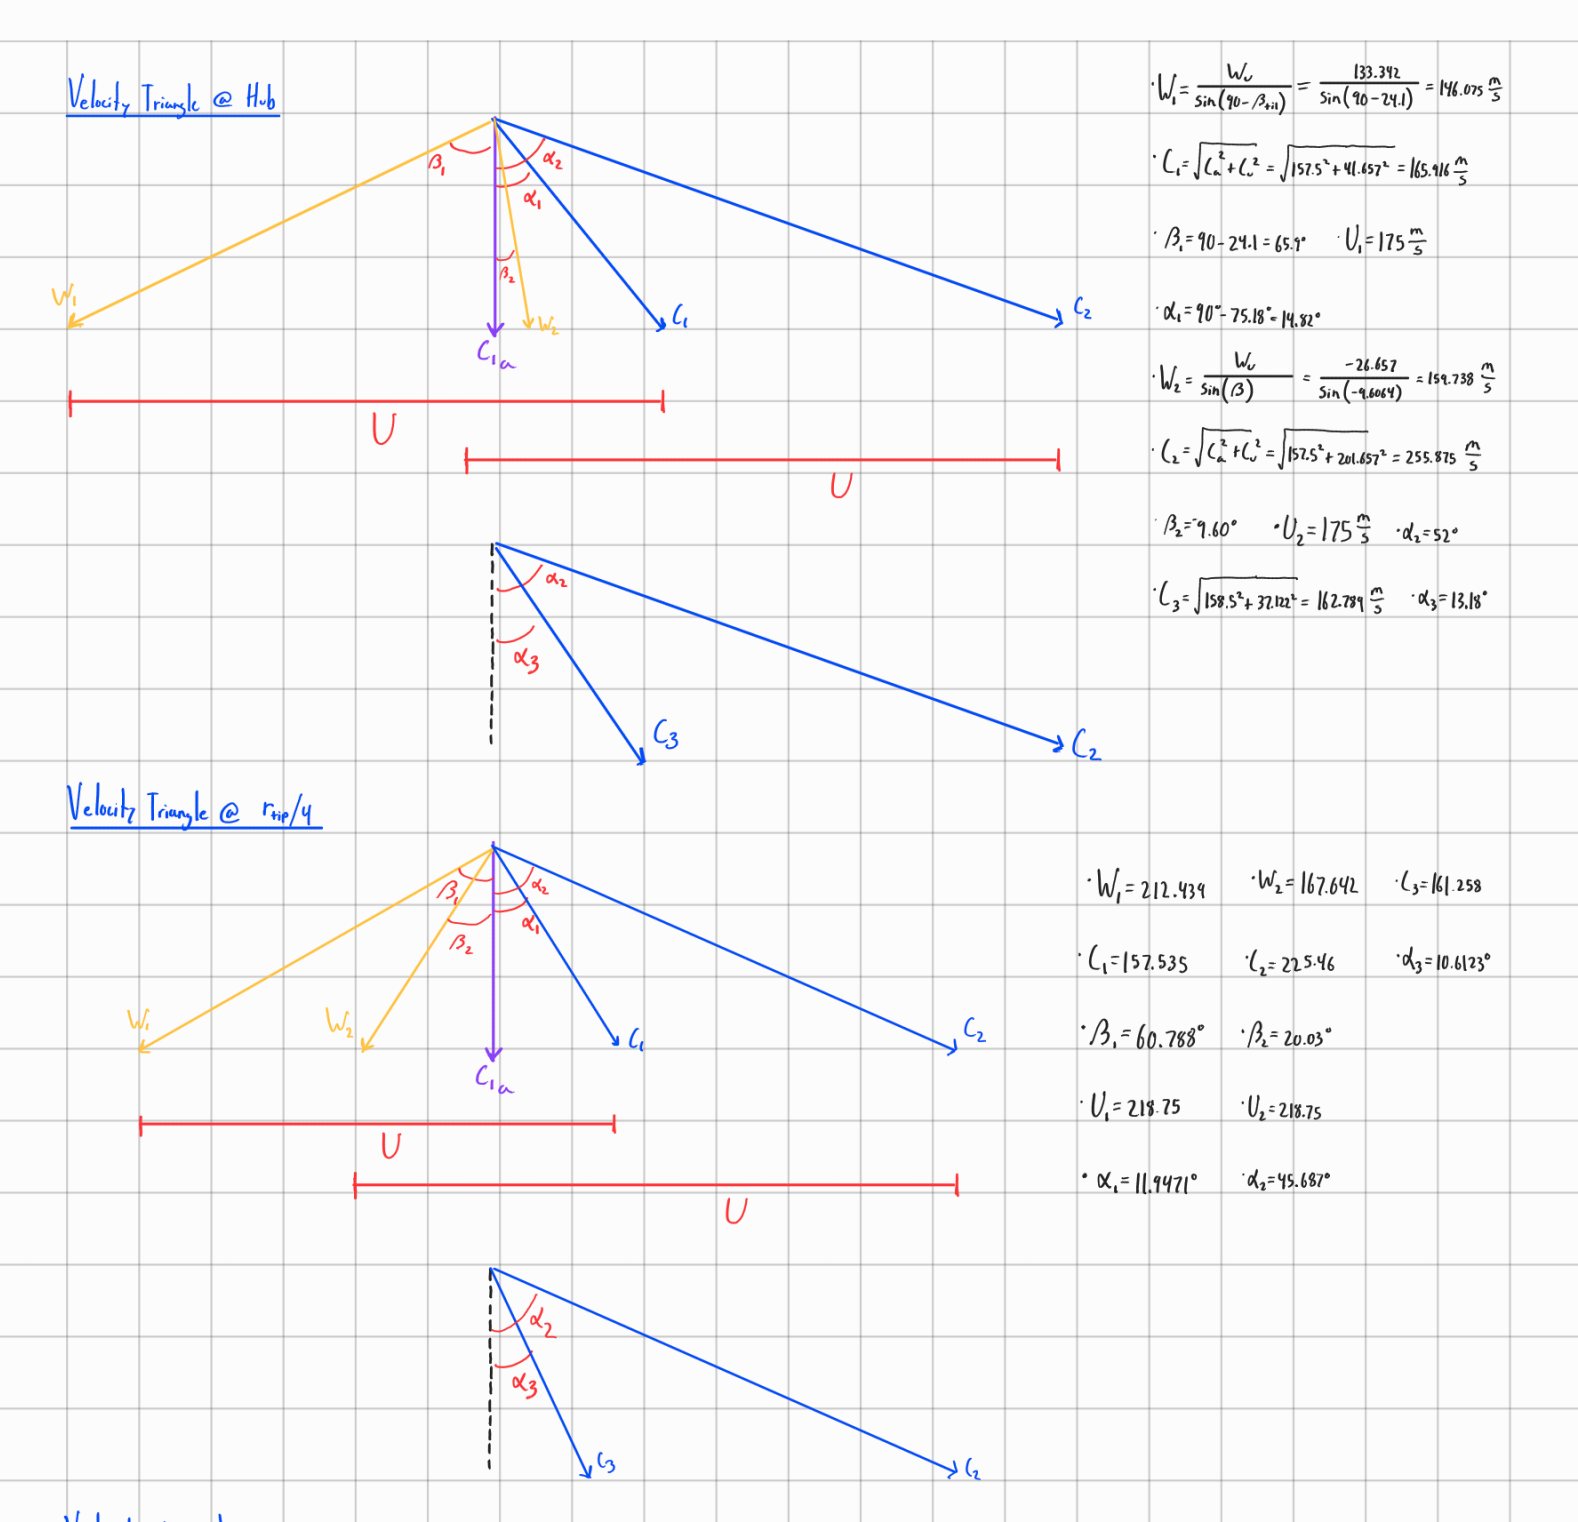
\includegraphics[width=0.75\textwidth]{veltri1.png}
    \end{center}

    \begin{center}
        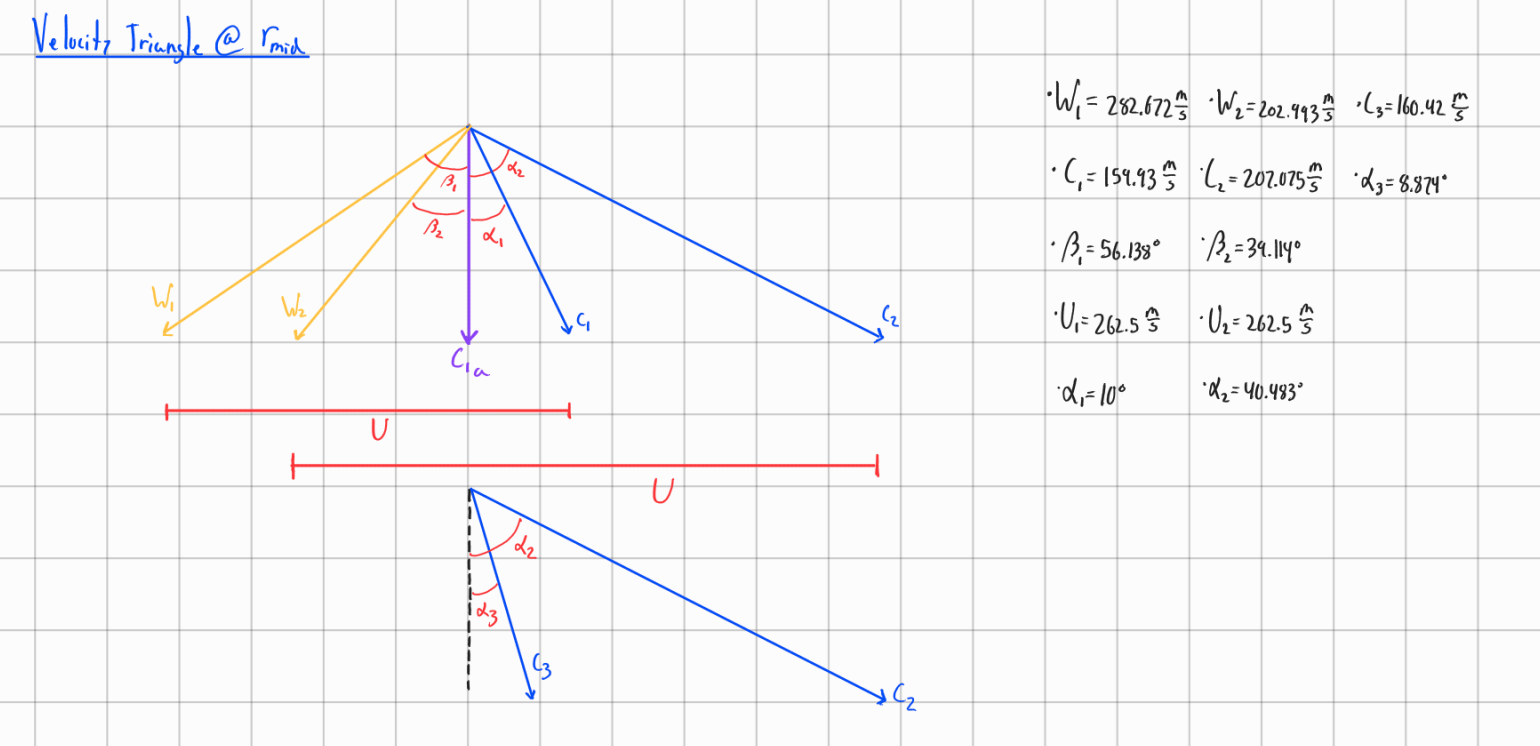
\includegraphics[width=0.75\textwidth]{veltri2.png}
    \end{center}

    \begin{center}
        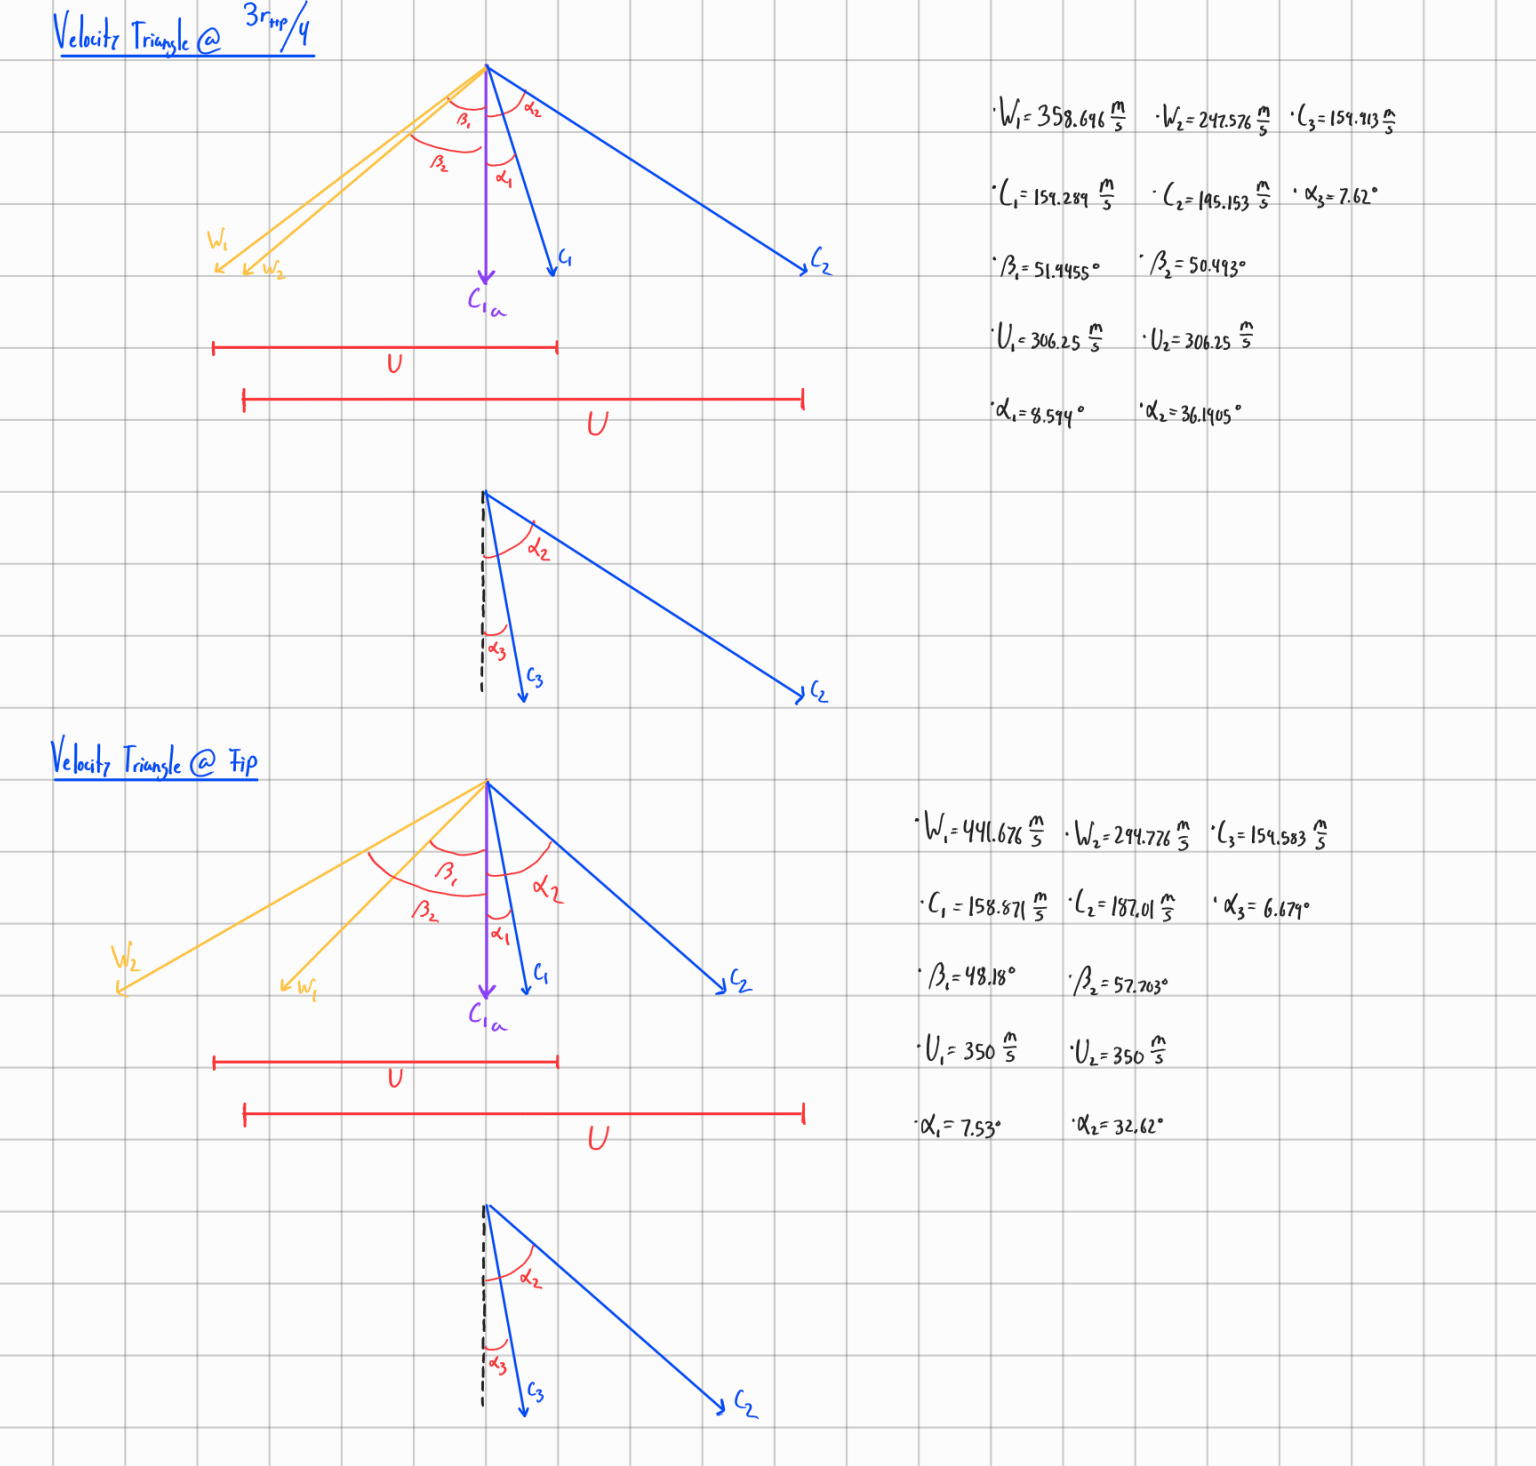
\includegraphics[width=0.75\textwidth]{veltri3.png}
    \end{center}
    

    \item Draw the rotor and stator airfoil stack for the camber line.
    
    \begin{center}
        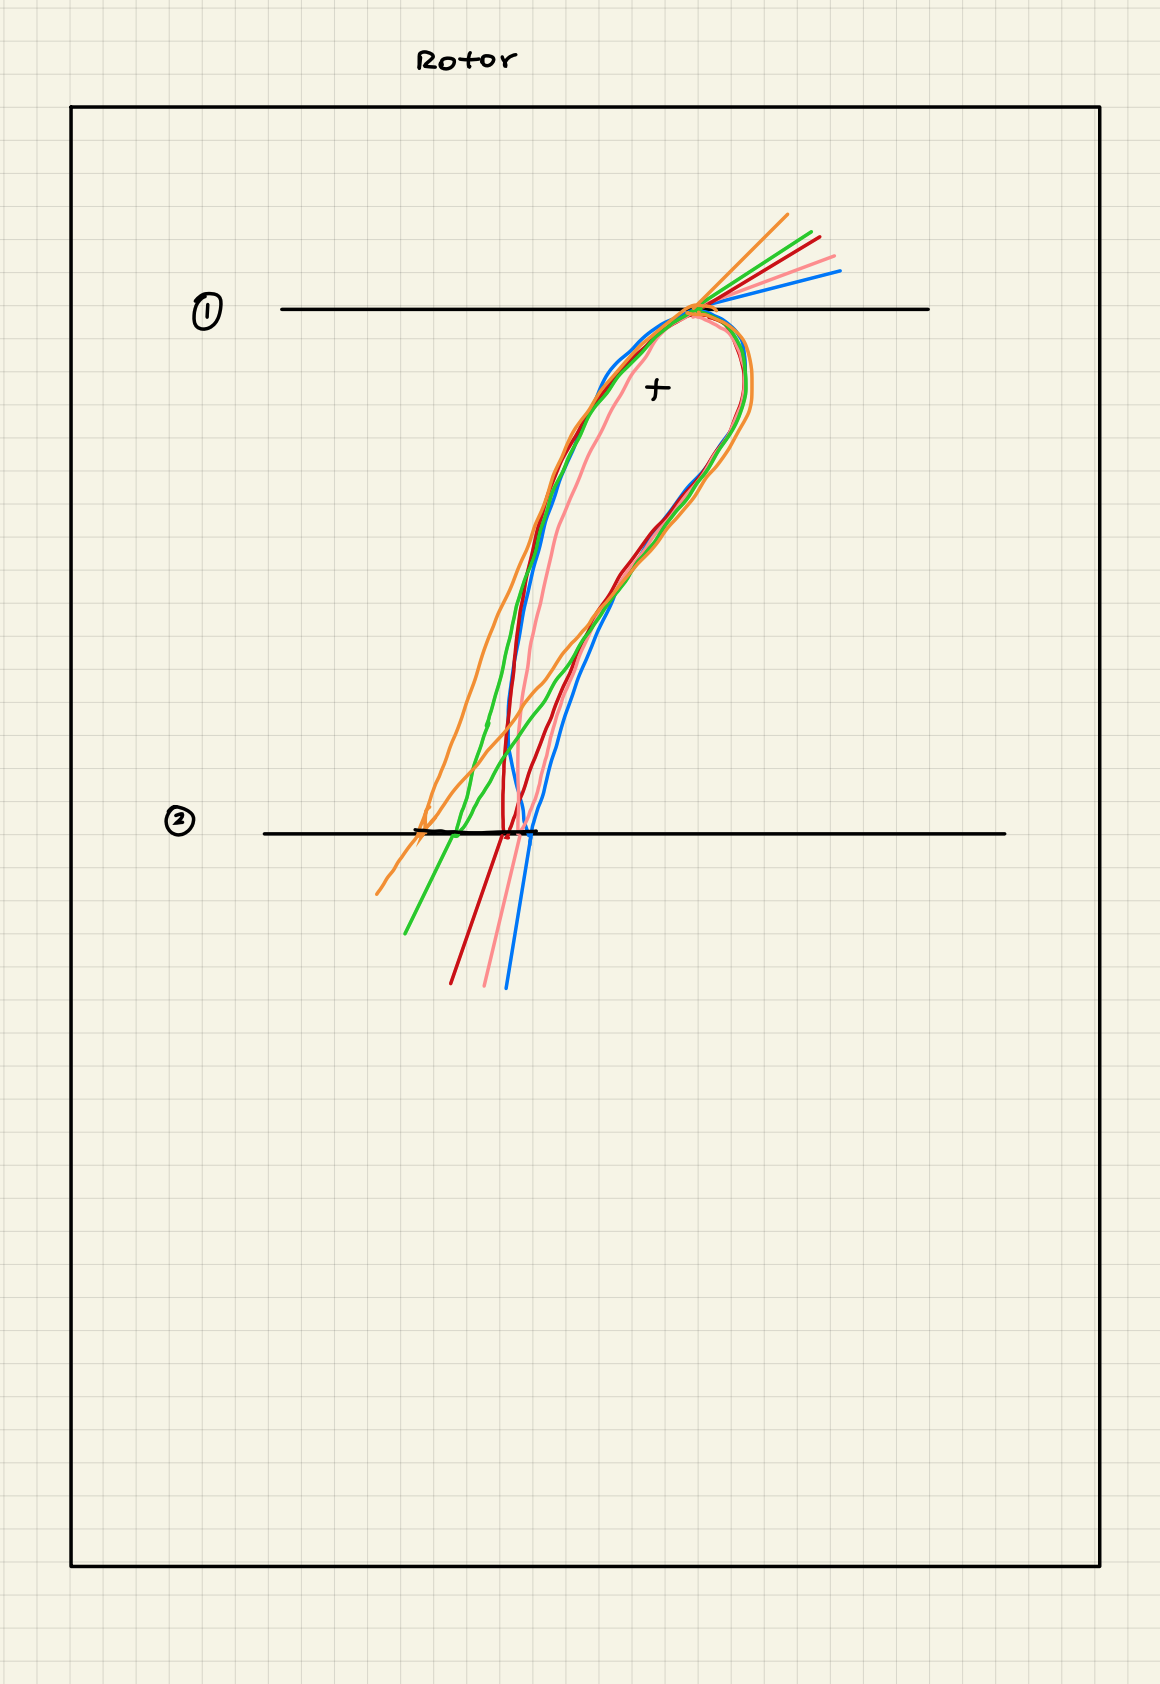
\includegraphics[width=0.75\textwidth]{airfoilstack.png}
    \end{center}

    \begin{center}
        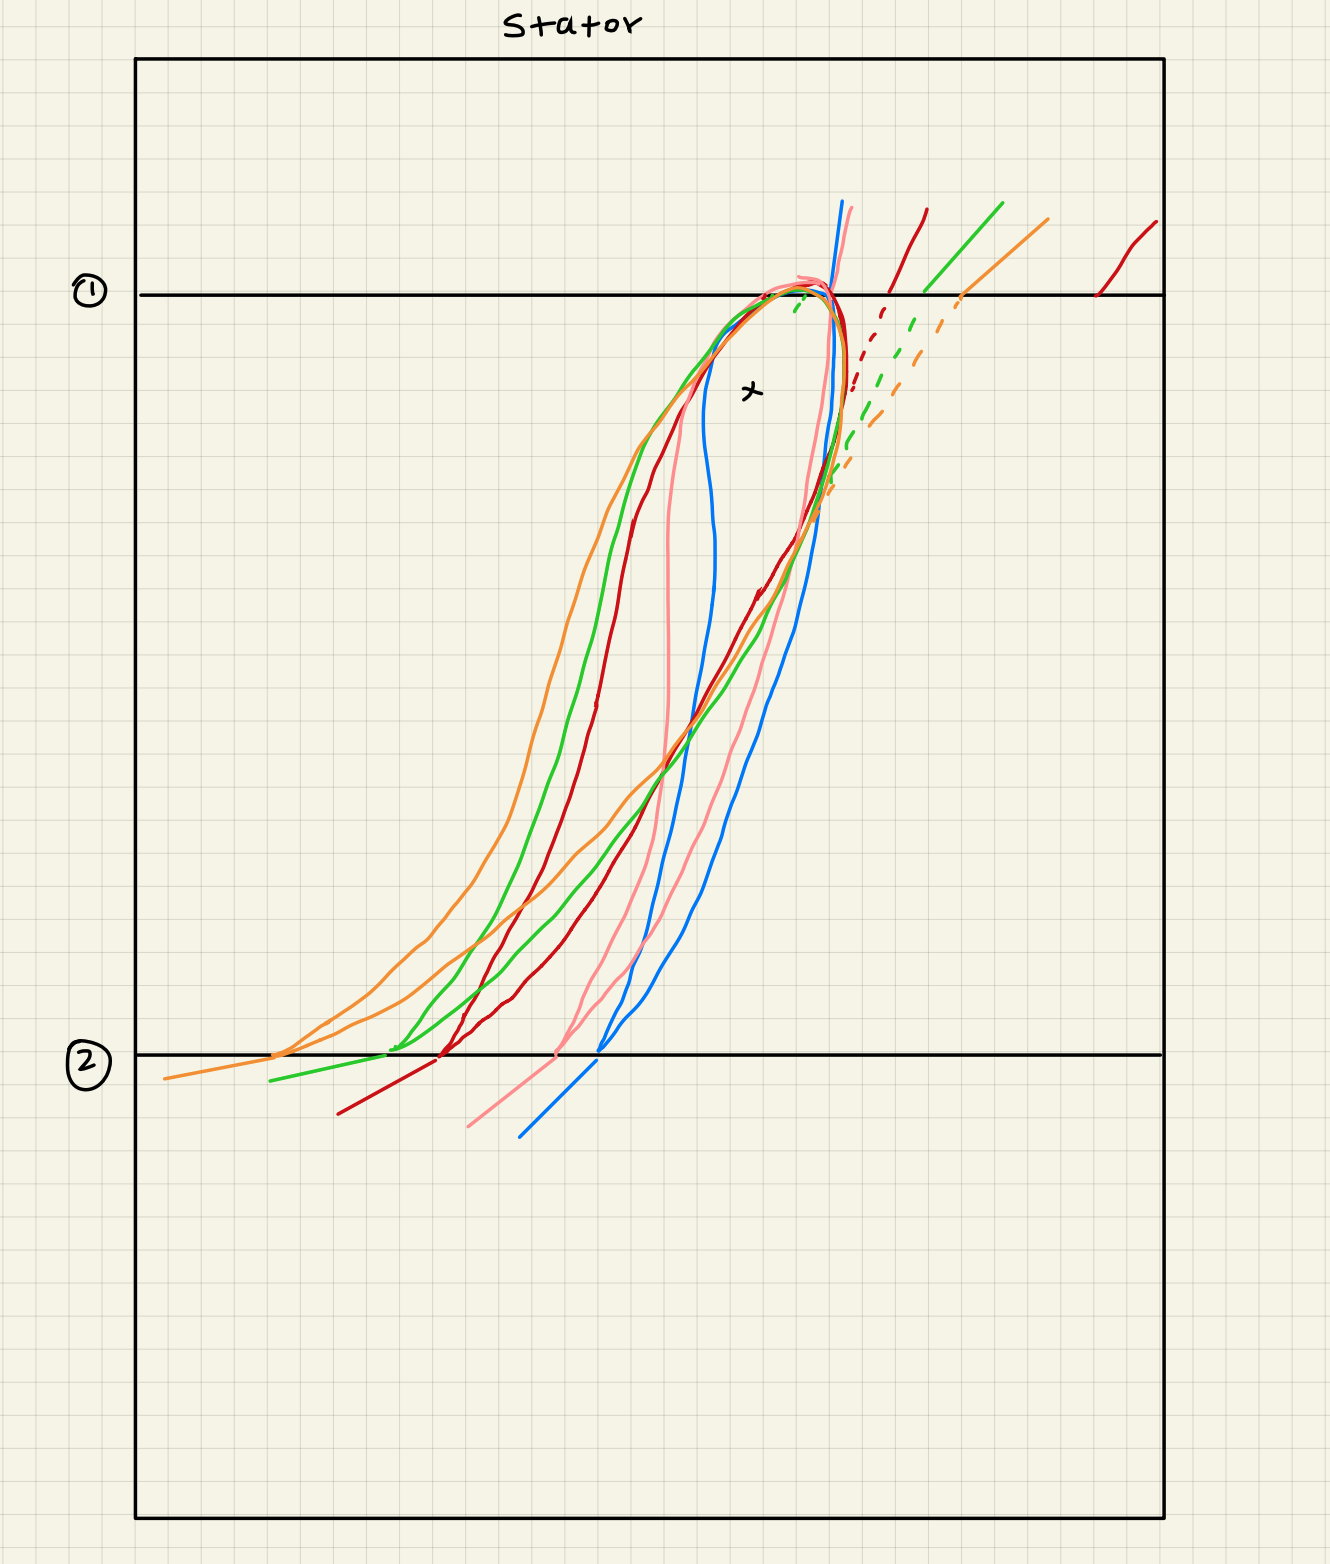
\includegraphics[width=0.75\textwidth]{airfoilstack2.png}
    \end{center}

\end{enumerate}

\vspace{7cm}

\section{Compressor Map - Task 4}

Input values:

\begin{equation}
    \dot{m} = 1.64089 \frac{kg}{s} 
\end{equation}

\begin{equation}
    \pi^{*}_{n} = 9.2
\end{equation}

\begin{equation}
    \eta = 0.89 
\end{equation}

\verb|task4_main.py| is the main file which calls the other files and runs the code. Readers are to run this code to perfom the analysis.

\vspace*{3pt}

\verb|Table2.1.csv| contains the data from Table 2.1 in Dr. Cizmas' notes. This data is used to calculate the values for the compressor map. This table is read in by \verb|task4_main.py| and is used to calculate the values for the compressor map. Table 2.1 is shown below:

\begin{center}
    \begin{tabular}{ c c c c c c c c c c }
     $\bar{n}$ & 0.5 & 0.6 & 0.7 & 0.8 & 0.9 & 1.0 & 1.05 & 1.1 \\ 
        $\bar{\eta_{base}}$ & 0.9 & 0.924 & 0.955 & 0.97 & 1.0 & 1.0 & 0.98 & 0.975 \\
        $\bar{\dot{m_{base}}}$ & 0.37 & 0.47 & 0.58 & 0.714 & 0.86 & 1.0 & 1.02 & 1.04 \\
        $\bar{\pi_{base}}$ & 0.47 & 0.51 & 0.59 & 0.7 & 0.82 & 1.0 & 1.1 & 1.2 \\
    \end{tabular}
    \end{center}

\vspace*{3pt}

Where; 
\begin{center}
    $\bar{n}$ = $\frac{n}{n_{ref}}$ 

    \vspace*{3pt}

    $\bar{\eta_{base}}$ = $\frac{\eta_{base}}{\eta_{ref}}$
    
    \vspace*{3pt}
    
    $\bar{\dot{m_{base}}}$ = $\frac{\dot{m_{base}}}{\dot{m_{ref}}}$
    
    \vspace*{3pt}
    
    $\bar{\pi_{base}}$ = $\frac{\pi^* _{base}}{\pi^* _{ref}}$
\end{center}

\vspace*{3pt}

\verb|Table2.3.csv| contains the data from Table 2.3 in Dr. Cizmas' notes. This data is used to calculate the values for the compressor map. This table is read in by \verb|task4_main.py| and is used to calculate the values for the compressor map. Table 2.3 is shown below:

\begin{center}
    \begin{tabular}{ c c c c c c c }
     $\frac{\bar{C_{a}}}{\bar{C_{a_{base}}}}$ & 0.8 & 0.9 & 1.0 & 1.1 & 1.2 \\ 
        $\frac{\eta}{\eta_{base}}$ & 0.92 & 0.98 & 1 & 0.97 & 0.88 \\
        $\frac{w}{w_{base}}$ & 1.25 & 1.12 & 1 & 0.9 & 0.82 \\ 
    \end{tabular}
    \end{center}

\vspace*{3pt}

Where;
\begin{equation}
    w = \frac{h^{*}_{1}}{\eta} (\pi^{* \frac{\gamma - 1}{\gamma}} - 1)
\end{equation}

\vspace*{3pt}

\begin{equation}
    h^{*}_{1} = \frac{w \eta}{\pi^{* \frac{\gamma - 1}{\gamma}} - 1}
\end{equation}

\vspace*{3pt}

Similarly we can say,

\begin{equation}
    h^{*}_{1} = \frac{w_{base} \eta_{base}}{(\pi^{* \frac{\gamma-1}{\gamma}})_{base} - 1}
\end{equation}

\vspace*{3pt}

Making use of these equations, we can write the following:

\begin{equation}
    \pi^{ * } = \left[ 1 + ((\pi^{ * \frac{\gamma - 1}{\gamma}})_{base} -1) \frac{w \eta}{w_{base} \eta_{base}} \right] ^{\frac{\gamma}{\gamma - 1}}
\end{equation}

\verb|steps.py| contains the 4 different steps that Dr. Cizmas has outlined in his notes. The steps are as follows:

\subsection{Compressor Map Algorithm}
\begin{enumerate}
    \item Calculate $\pi^{*} = \pi^{*} (\bar{n}, \frac{\bar{C_{a}}}{\bar{C_{a_{base}}}})$ and $\frac{\pi^{*}}{\pi^{*}_{base} = f (\bar{n}, \frac{\bar{C_{a}}}{\bar{C_{a_{base}}}})}$, where where $\bar{n} \in (0.5, 1.1)$ and $\frac{\bar{C_a}}{\bar{C_{a base}}} \in (0.8, 1.2)$ producing a table as shown in Table 2.4.1 and Table 2.4.2. (Tables are in \verb|Table_2_4_1.csv| and \verb|Table_2_4_2.csv| respectively)
    \begin{center}
        \begin{tabular}{ c c c c c c c c }
            $\frac{\bar{C_{a}}}{\bar{C_{a_{base}}}}$ & 0.8 & 0.9 & 1.0 & 1.1 & 1.2 & $\bar{n}$ \\
            $\pi^{*}$ & 4.64045 & 4.38299 & 3.93091 & 3.39379 & 2.83897 & 0.5 \\
            $\pi^{*}$ & 5.07483 & 4.78063 & 4.26545 & 3.65607 & 3.03024 & 0.6 \\
            $\pi^{*}$ & 5.95028 & 5.57996 & 4.93454 & 4.17687 & 3.40661 & 0.7 \\
            $\pi^{*}$ & 7.16637 & 6.68649 & 5.85454 & 4.88616 & 3.91291 & 0.8 \\
            $\pi^{*}$ & 8.50639 & 7.90169 & 6.85818 & 5.65264 & 4.45332 & 0.9 \\
            $\pi^{*}$ & 10.5374 & 9.73710 & 8.36364 & 6.79104 & 5.24562 & 1.0 \\
            $\pi^{*}$ & 11.6748 & 10.7622 & 9.19999 & 7.41866 & 5.67803 & 1.05 \\
            $\pi^{*}$ & 12.8177 & 11.7906 & 10.0363 & 8.04337 & 6.10576 & 1.1 \\
        \end{tabular}

        \vspace*{3pt}

        \begin{tabular}{c c c c c c c c }
            $\frac{\bar{C_{a}}}{\bar{C_{a_{base}}}}$ & 0.8 & 0.9 & 1.0 & 1.1 & 1.2 & $\bar{n}$ \\
            $\frac{\pi^{*}}{\pi^{*}_{base}}$ & 1.18050 & 1.11501 & 0.99999 & 0.86336 & 0.72222 & 0.5 \\
            $\frac{\pi^{*}}{\pi^{*}_{base}}$ & 1.18975 & 1.12078 & 0.99999 & 0.85713 & 0.71042 & 0.6 \\
            $\frac{\pi^{*}}{\pi^{*}_{base}}$ & 1.20584 & 1.13079 & 1.0 & 0.84646 & 0.69036 & 0.7 \\
            $\frac{\pi^{*}}{\pi^{*}_{base}}$ & 1.22407 & 1.14210 & 0.99999 & 0.83459 & 0.66835 & 0.8 \\
            $\frac{\pi^{*}}{\pi^{*}_{base}}$ & 1.24033 & 1.15215 & 0.99999 &  0.82422 & 0.64934 & 0.9 \\
            $\frac{\pi^{*}}{\pi^{*}_{base}}$ & 1.25991 & 1.16422 & 1.0 & 0.81197 & 0.62719 & 1.0 \\
            $\frac{\pi^{*}}{\pi^{*}_{base}}$ & 1.26899 & 1.16980 & 0.99999 & 0.80638 & 0.617177 & 1.05 \\
            $\frac{\pi^{*}}{\pi^{*}_{base}}$ & 1.27712 & 1.17479 & 0.99999 & 0.80142 & 0.608364 & 1.1 \\
        \end{tabular}
    \end{center}

    \item Calculate $\frac{\bar{\dot{m}}}{\bar{\dot{m_{base}}}} = f (\bar{n}, \frac{\bar{C_{a}}}{\bar{C_{a_{base}}}})$, by making use of:
    
    \begin{equation}
        \frac{\bar{\dot{m}}}{\bar{\dot{m_{base}}}} = \frac{\bar{C_{a}}}{\bar{C_{a_{base}}}} \left[ \frac{\bar{\pi^{*}}}{\bar{\pi^{*}_{base}}} \right] ^{\frac{1}{3}}
    \end{equation}

    Similar to step 1. Table 2.5 is produced. (Table is in \verb|Table_2_5_csv|)

    \begin{center}
        \begin{tabular}{ c c c c c c c c }
            $\frac{\bar{C_{a}}}{\bar{C_{a_{base}}}}$ & 0.8 & 0.9 & 1.0 & 1.1 & 1.2 & $\bar{n}$ \\
            $\frac{\bar{\dot{m}}}{\bar{\dot{m_{base}}}}$ & 0.84549 & 0.93326 & 1.0 & 1.04743 & 1.07664 & 0.5 \\
            $\frac{\bar{\dot{m}}}{\bar{\dot{m_{base}}}}$ & 0.84769 & 0.93487 & 0.99999 & 1.04490 & 1.07074 & 0.6 \\
            $\frac{\bar{\dot{m}}}{\bar{\dot{m_{base}}}}$ & 0.85150 & 0.93764 & 1.0 & 1.04054 & 1.06057 & 0.7 \\
            $\frac{\bar{\dot{m}}}{\bar{\dot{m_{base}}}}$ & 0.85577 & 0.94076 & 0.99999 & 1.03566 & 1.04918 & 0.8 \\
            $\frac{\bar{\dot{m}}}{\bar{\dot{m_{base}}}}$ & 0.85955 & 0.94351 & 1.0 & 1.03135 & 1.03914 & 0.9 \\
            $\frac{\bar{\dot{m}}}{\bar{\dot{m_{base}}}}$ & 0.86404 & 0.94679 & 1.0 & 1.02622 & 1.02718 & 1.0 \\
            $\frac{\bar{\dot{m}}}{\bar{\dot{m_{base}}}}$ & 0.86612 & 0.94830 & 0.99999 & 1.02386 & 1.02169 & 1.05 \\
            $\frac{\bar{\dot{m}}}{\bar{\dot{m_{base}}}}$ & 0.86796 & 0.94965 & 0.99999 & 1.02175 & 1.01680 & 1.1 \\
        \end{tabular}
    \end{center}

    \item Calculate $\bar{\pi} = \bar{\pi} (\bar{n}, \frac{\bar{C_{a}}}{\bar{C_{a_{base}}}})$ and $\bar{\dot{m}} = \bar{\dot{m}} (\bar{n}, \frac{\bar{C_{a}}}{\bar{C_{a_{base}}}})$, by making use of:
    \begin{equation}
        \bar{\pi} = \bar{\pi_{base}} \frac{\pi^{*}}{\pi^{*}_{base}}
    \end{equation}

    Where $\bar{pi_{base}}$ comes from \verb|Table2.1.csv| and $\frac{\pi^{*}}{\pi^{*}_{base}}$ comes from \verb|Table_2_4_2.csv|. Similarly,
    \begin{equation}
        \bar{\dot{m}} = \bar{\dot{m_{base}}} \frac{\bar{\dot{m}}}{\bar{\dot{m_{base}}}}
    \end{equation}

    Where $\bar{\dot{m_{base}}}$ comes from \verb|Table2.1.csv| and $\frac{\bar{\dot{m}}}{\bar{\dot{m_{base}}}}$ comes from \verb|Table_2_5.csv|. 

    \item Calculate $\eta = \eta (\bar{n}, \frac{\bar{C_{a}}}{\bar{C_{a_{base}}}})$ using tables \verb|Table2.1.csv|, \verb|Table2.3.csv|.
    
    \item Lastly we are to draw the Compressor map, with axes of $\dot{m} \frac{\sqrt{T^{*}_{1}}}{p^{*}_{1}}$, $\pi^{*}$ and $\eta$. We also provide a drawing of the surge line. The map is drawn:
    
    \begin{center}
        % include the image but fit it to the page
        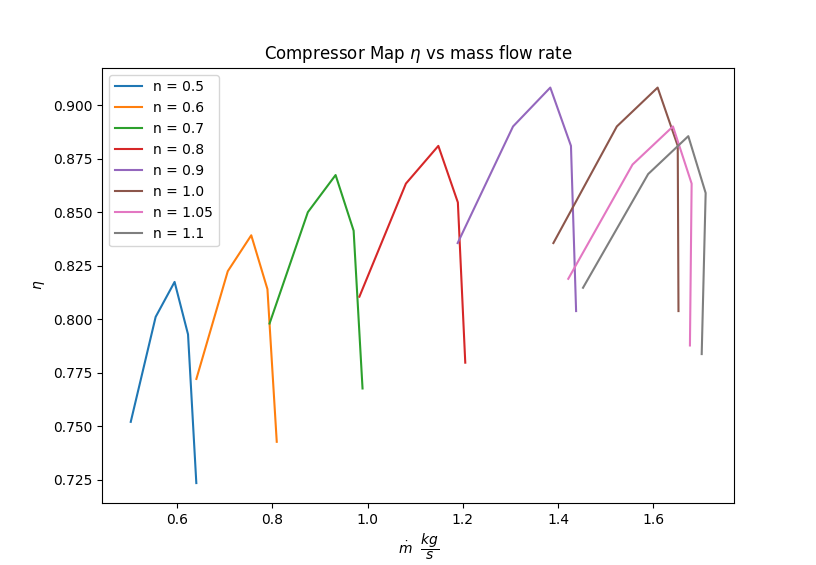
\includegraphics[width=\textwidth]{CompressorMap1.png}

    
        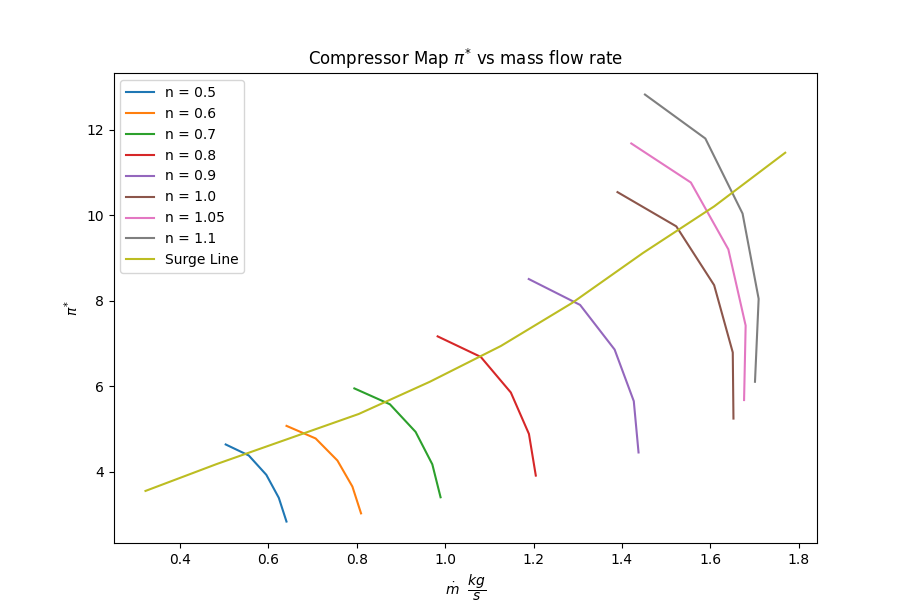
\includegraphics[width=\textwidth]{CompressorMap2.png}

        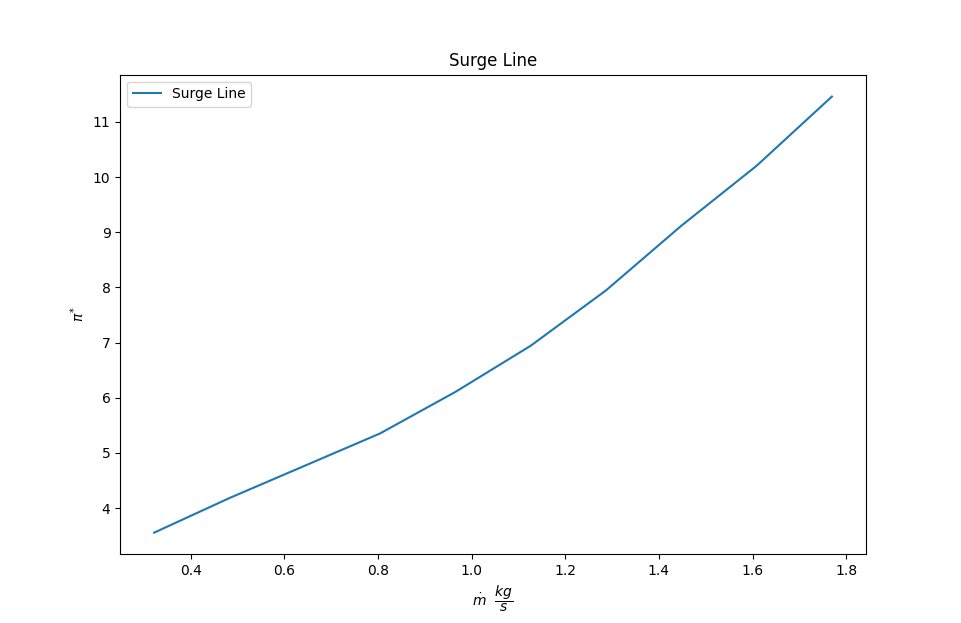
\includegraphics[width=\textwidth]{CompressorMap3.png}

    \end{center}
\end{enumerate}

\section{Compressor Airfoil CFD - Task 5}

\subsection{Overview}
This section contains the results of the CFD analysis performed on the compressor airfoil our team has chosen from Task 3.

\subsection{Flow Conditions}
As defined in the \textit{T.L. User's Manual}, the flow through a cascade is defined by two parameters:
\begin{itemize}
\item The inlet flow Mach number $M_{in}$
\item inlet flow angle $\alpha_{in}$
\end{itemize}

We have two non-dimensional parameters that define the flow through the cascade:

\begin{equation}
\label{eq:non-dim rho}
\rho_{in} = 1
\end{equation}

\begin{equation}
\label{eq:non-dim v}
V_{in} = 1
\end{equation}

Where, $\rho_{in}$ is the static density at the inlet and $V_{in}$ is the velocity at the inlet.  
From here we can calculate the Mach number at the inlet:

\begin{equation}
\label{eq:inlet mach}
M_{in} = \frac{V_{in}}{c_{in}}
\end{equation}

Since $V_{in}$ is a non-dimensional parameter, we need to non-dimensionalize the speed of sound $c_{in}$. 
We can do this by taking a look at how $V_{in}$ is defined:

\begin{equation}
\label{eq:def inlet velocity}
V_{in} = \frac{157.5}{157.5}
\end{equation}

Applying the same logic to the speed of sound we get:

\begin{equation}
\label{eq:def inlet speed of sound}
c_{in} = \frac{\sqrt{\gamma R T}}{157.5}
\end{equation}

Where $\gamma$ is the ratio of specific heats, $R$ is the gas constant and $T$ is the temperature.
Since this all takes place in the compressor, the working fluid is air, meaning that $\gamma = 1.4$
and $R = 287.058 \frac{J}{kgK}$.

Resulting in our Mach number to be:

\begin{equation}
\label{eq:mach}
M_{in} = 0.462823
\end{equation}

We are then able to calculate the static pressure at the inlet:

\begin{equation}
\label{eq:inlet pressure}
p_{in} = \frac{1}{\gamma M_{in}^2}
\end{equation}

Readers may recall the standard isentropic relations for pressure and density from AERO 201:

\begin{equation}
\label{eq:isentropic pressure}
p_{0} = p \left( 1 + \frac{\gamma-1}{2} M^{2} \right)^{\frac{\gamma}{\gamma - 1}}
\end{equation}

\begin{equation}
\label{eq:isentropic density}
\rho_{0} = \rho \left( 1 + \frac{\gamma-1}{2} M^{2} \right)^{\frac{1}{\gamma - 1}}
\end{equation}

We can makew use of these relations to calculate the total pressure and density at the inlet:

\begin{equation}
\label{eq:total pressure}
p_{0_{in}} = p_{in} \left( 1 + \frac{\gamma-1}{2} M_{in}^{2} \right)^{\frac{\gamma}{\gamma - 1}}
\end{equation}

\begin{equation}
\label{eq:total density}
\rho_{0_{in}} = \rho_{in} \left( 1 + \frac{\gamma-1}{2} M_{in}^{2} \right)^{\frac{1}{\gamma - 1}}
\end{equation}

We calculated our total parameters to be:

\begin{equation}
\label{eq:total pressure}
p_{0_{in}} = 2.87924668
\end{equation}

\begin{equation}
\label{eq:total density}
\rho_{0_{in}} = 0.9004399
\end{equation}

We induced a flow angle of $\alpha_{in} = 44.6$ degrees. 
Alowing for us to calculate the:

\begin{equation}
\label{eq:FLUX}
\verb|FLUX| = V_{in} \cos{\alpha_{in}}
\end{equation}

\begin{equation}
\label{eq:VTAN}
\verb|VTAN| = V_{in} \sin{\alpha_{in}}
\end{equation}

Resulting in:

\begin{center}
  $\verb|FLUX| = 0.712026045991$ \\
  $\verb|VTAN| = 0.702153052995$ \\
  $\verb|UINIT| = 0.712026045991$ \\
  $\verb|VINIT| = 0.702153052995$ \\
\end{center}

\subsection{Computational Fluid Dynamics Figures}

\begin{center}
    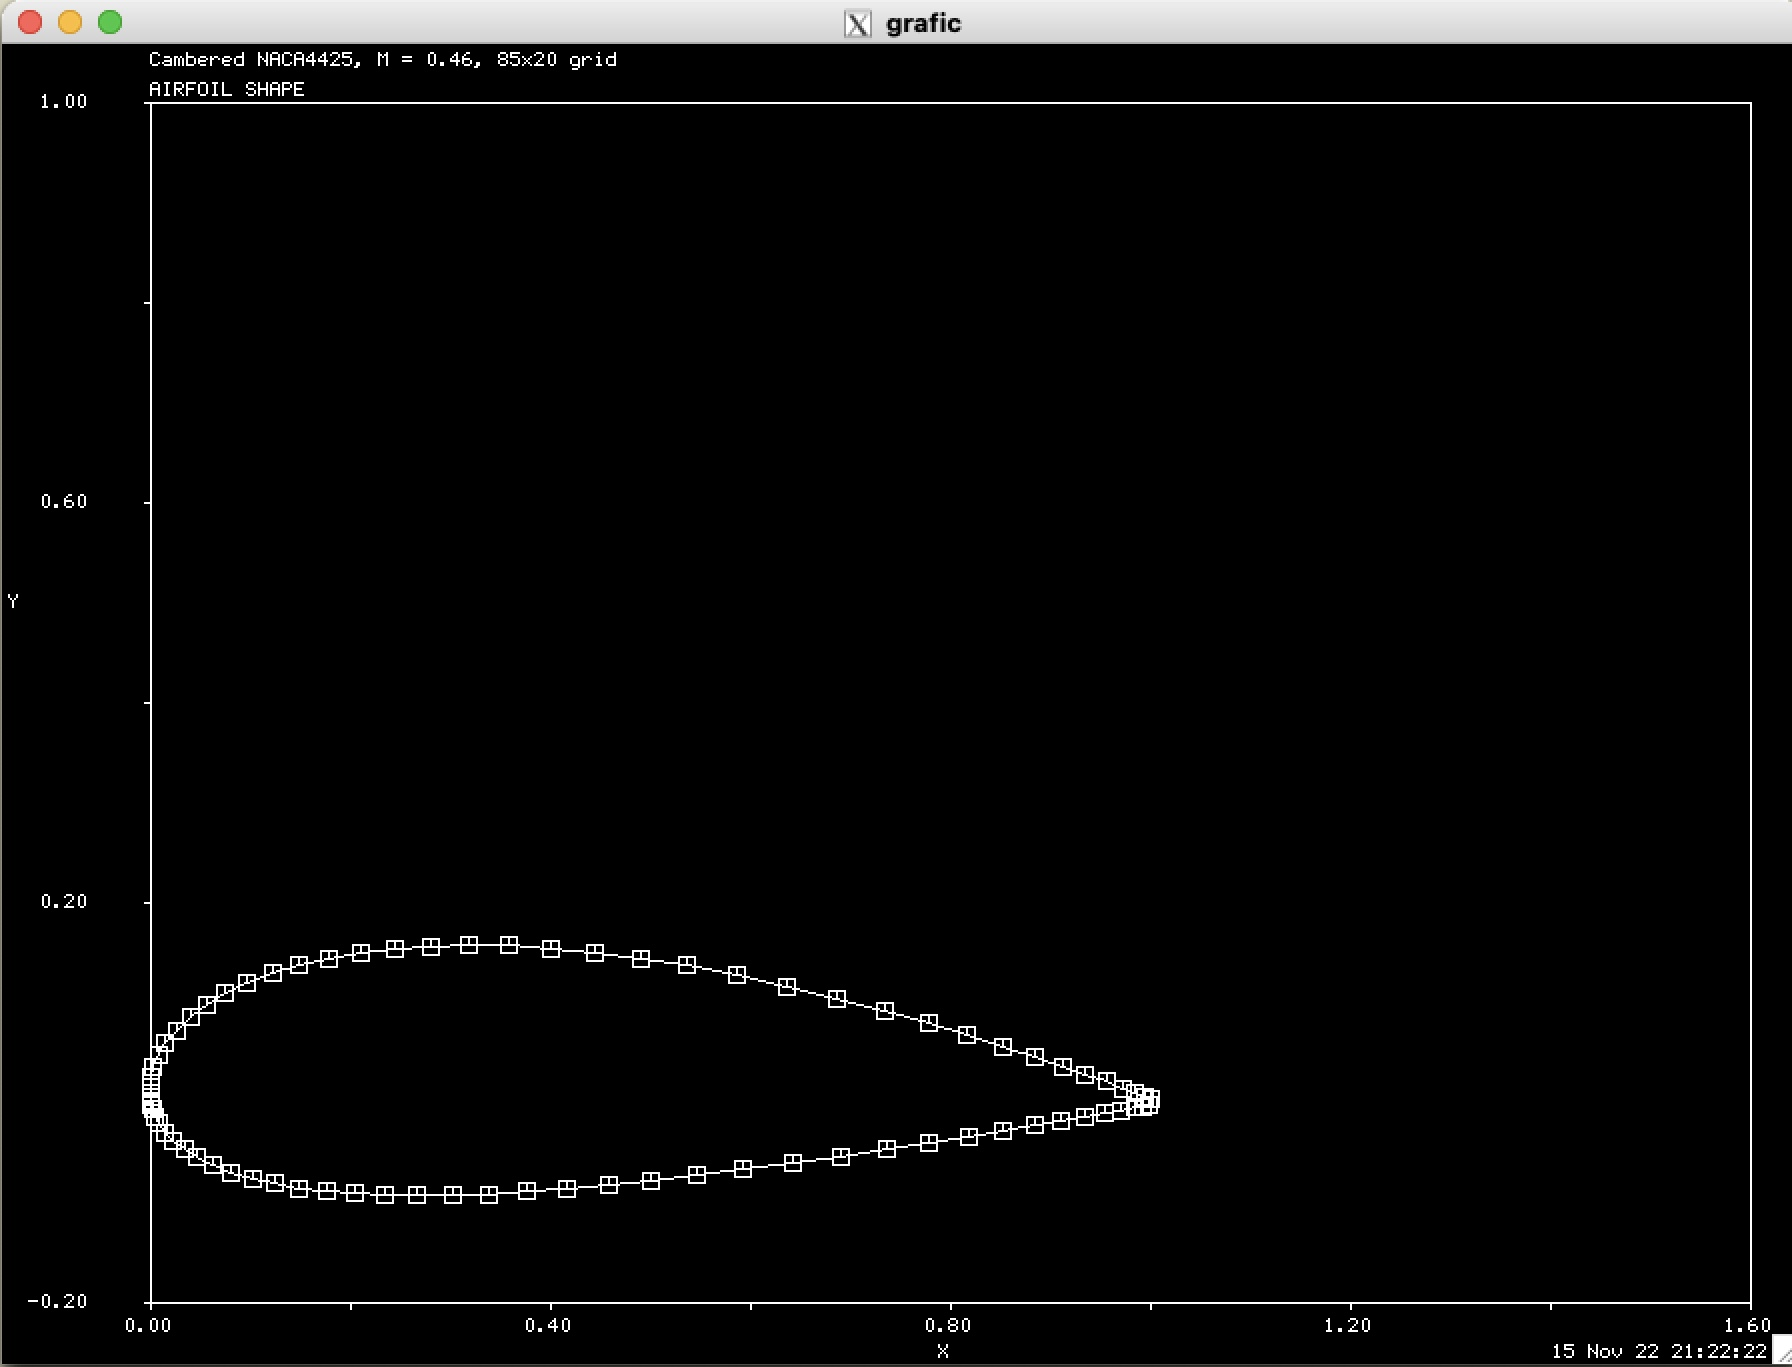
\includegraphics[width=0.75\textwidth]{/airfoil1.jpeg}
\end{center}

\begin{center}
  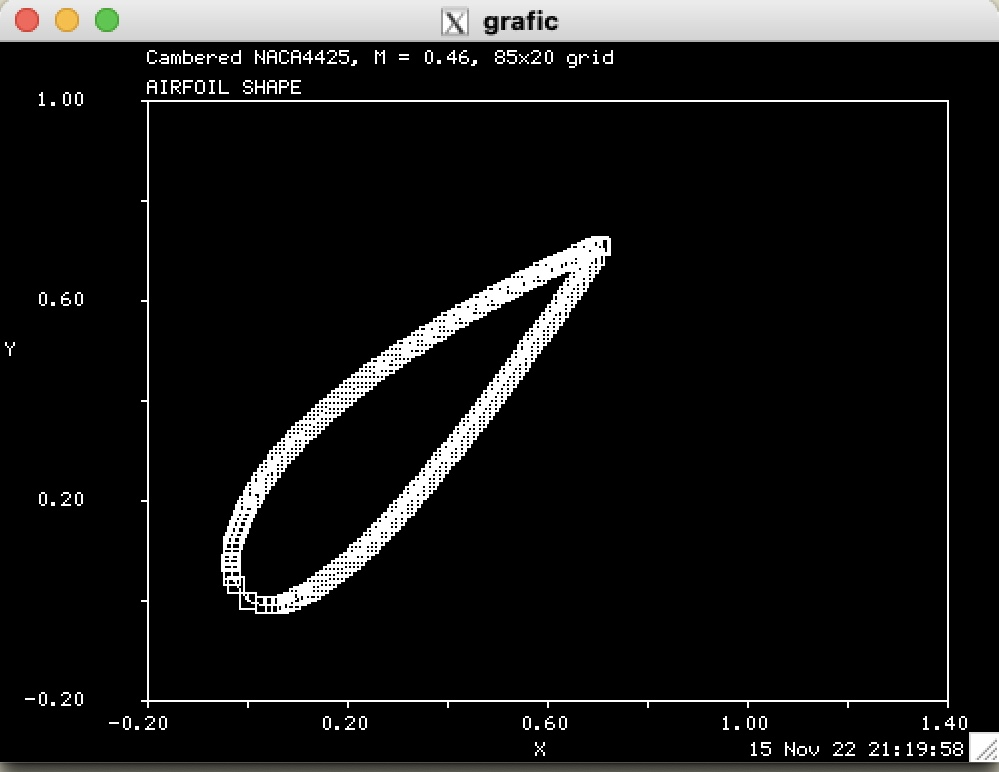
\includegraphics[width=0.75\textwidth]{/airfoil2.jpeg}
\end{center}

\begin{center}
  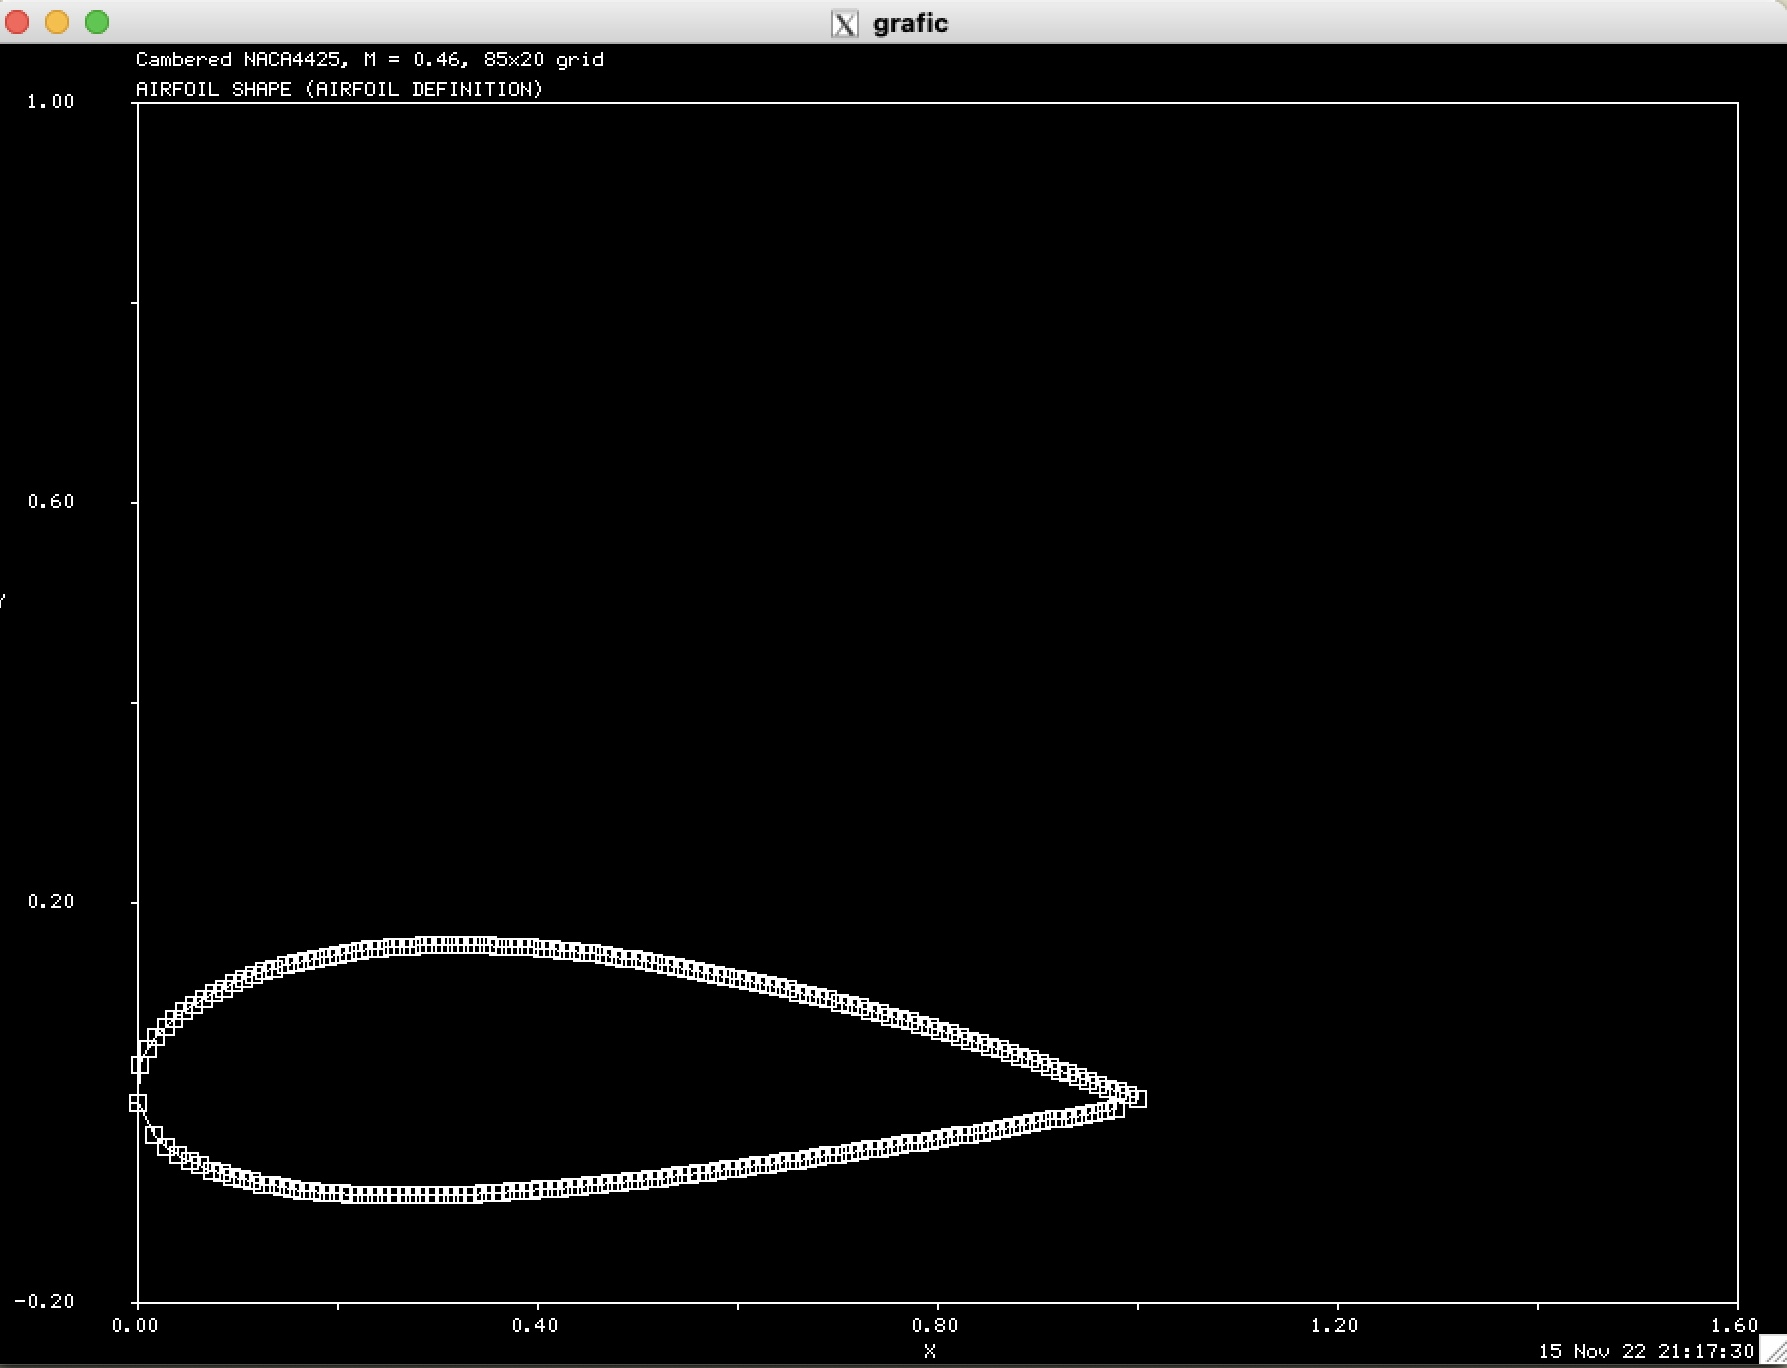
\includegraphics[width=0.75\textwidth]{/airfoil3.jpeg}
\end{center}

\begin{center}
  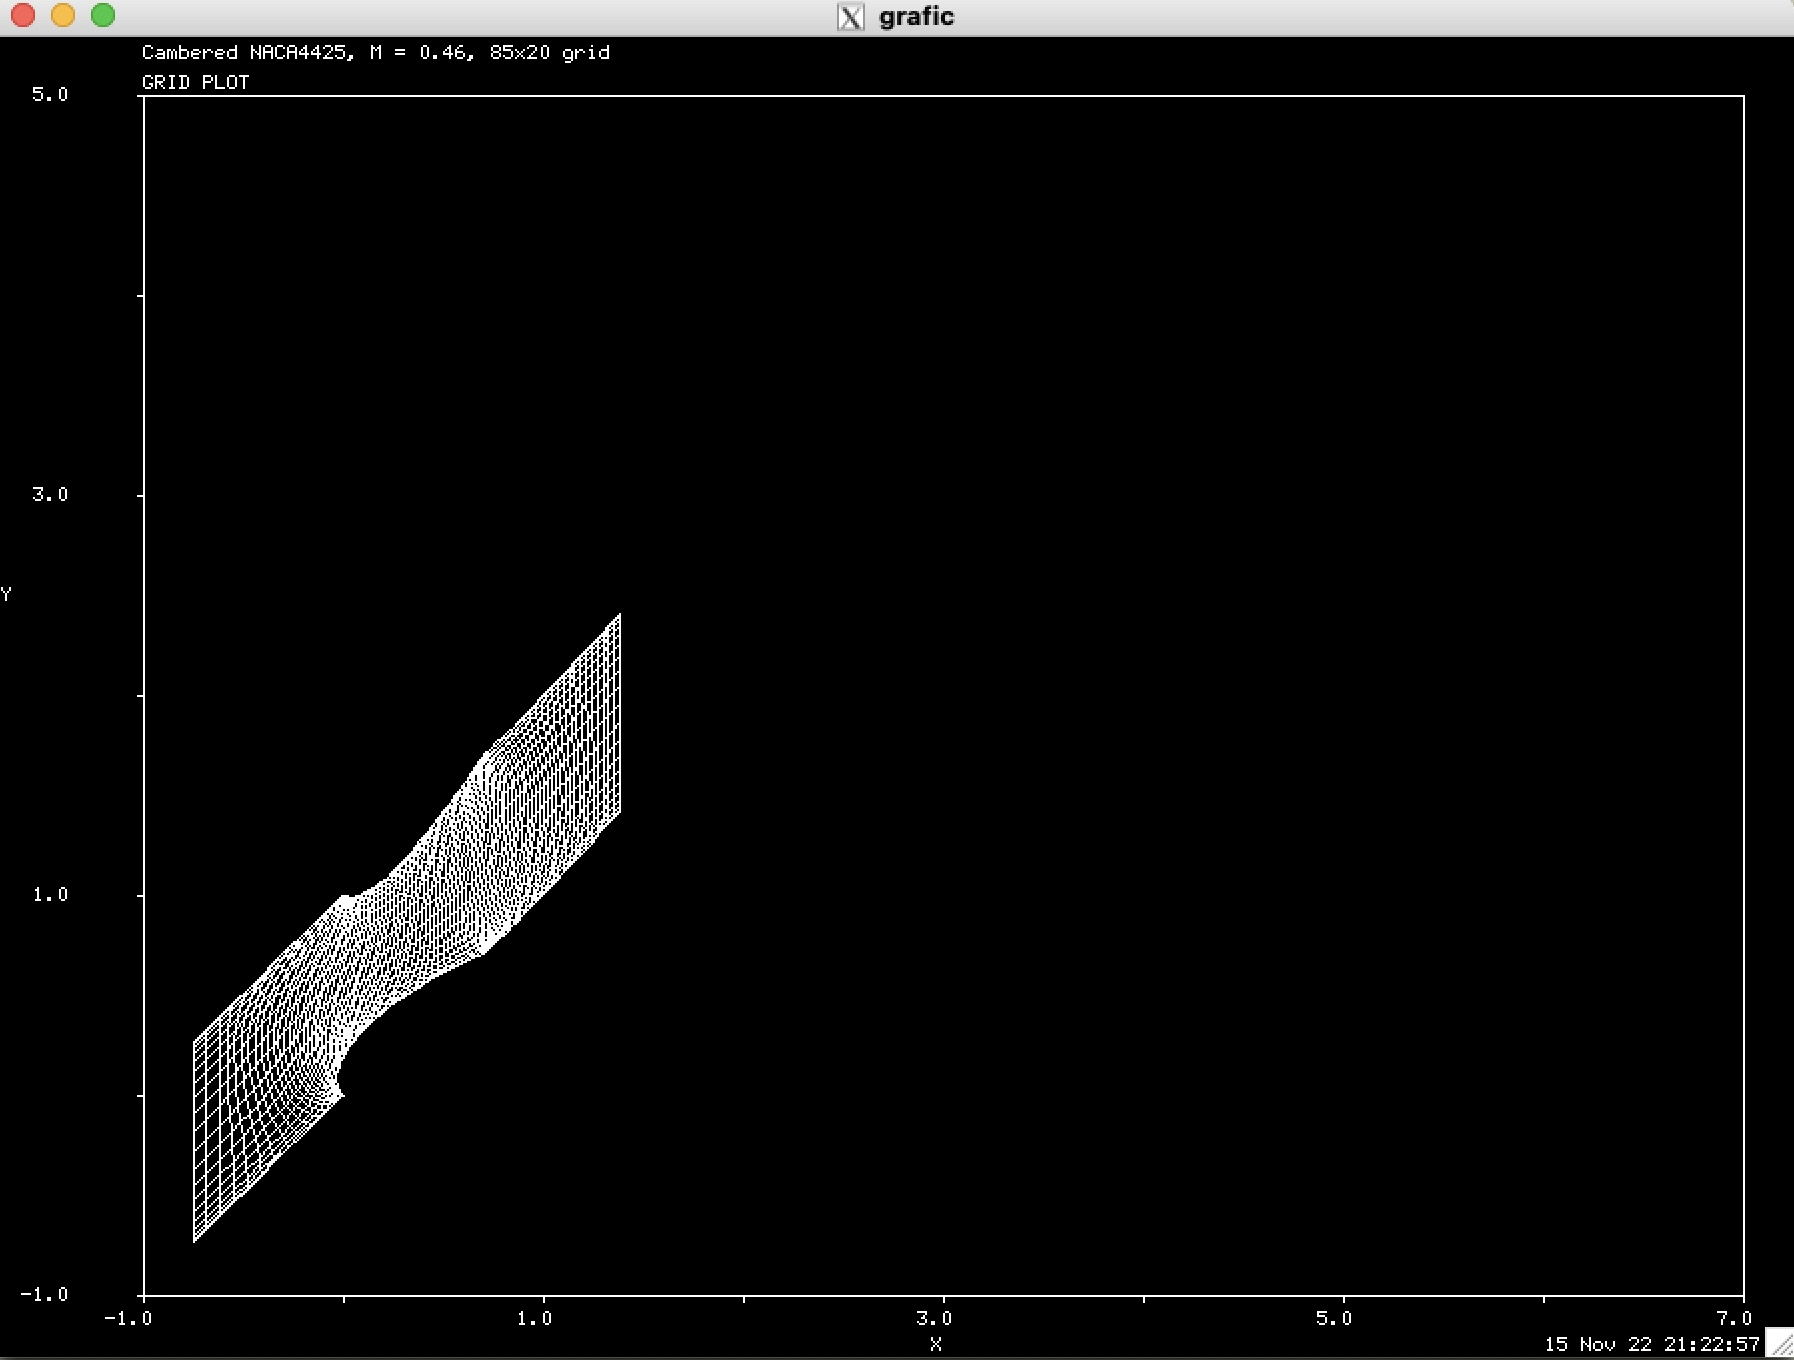
\includegraphics[width=0.75\textwidth]{/compgrid.jpeg}
\end{center}

\begin{center}
  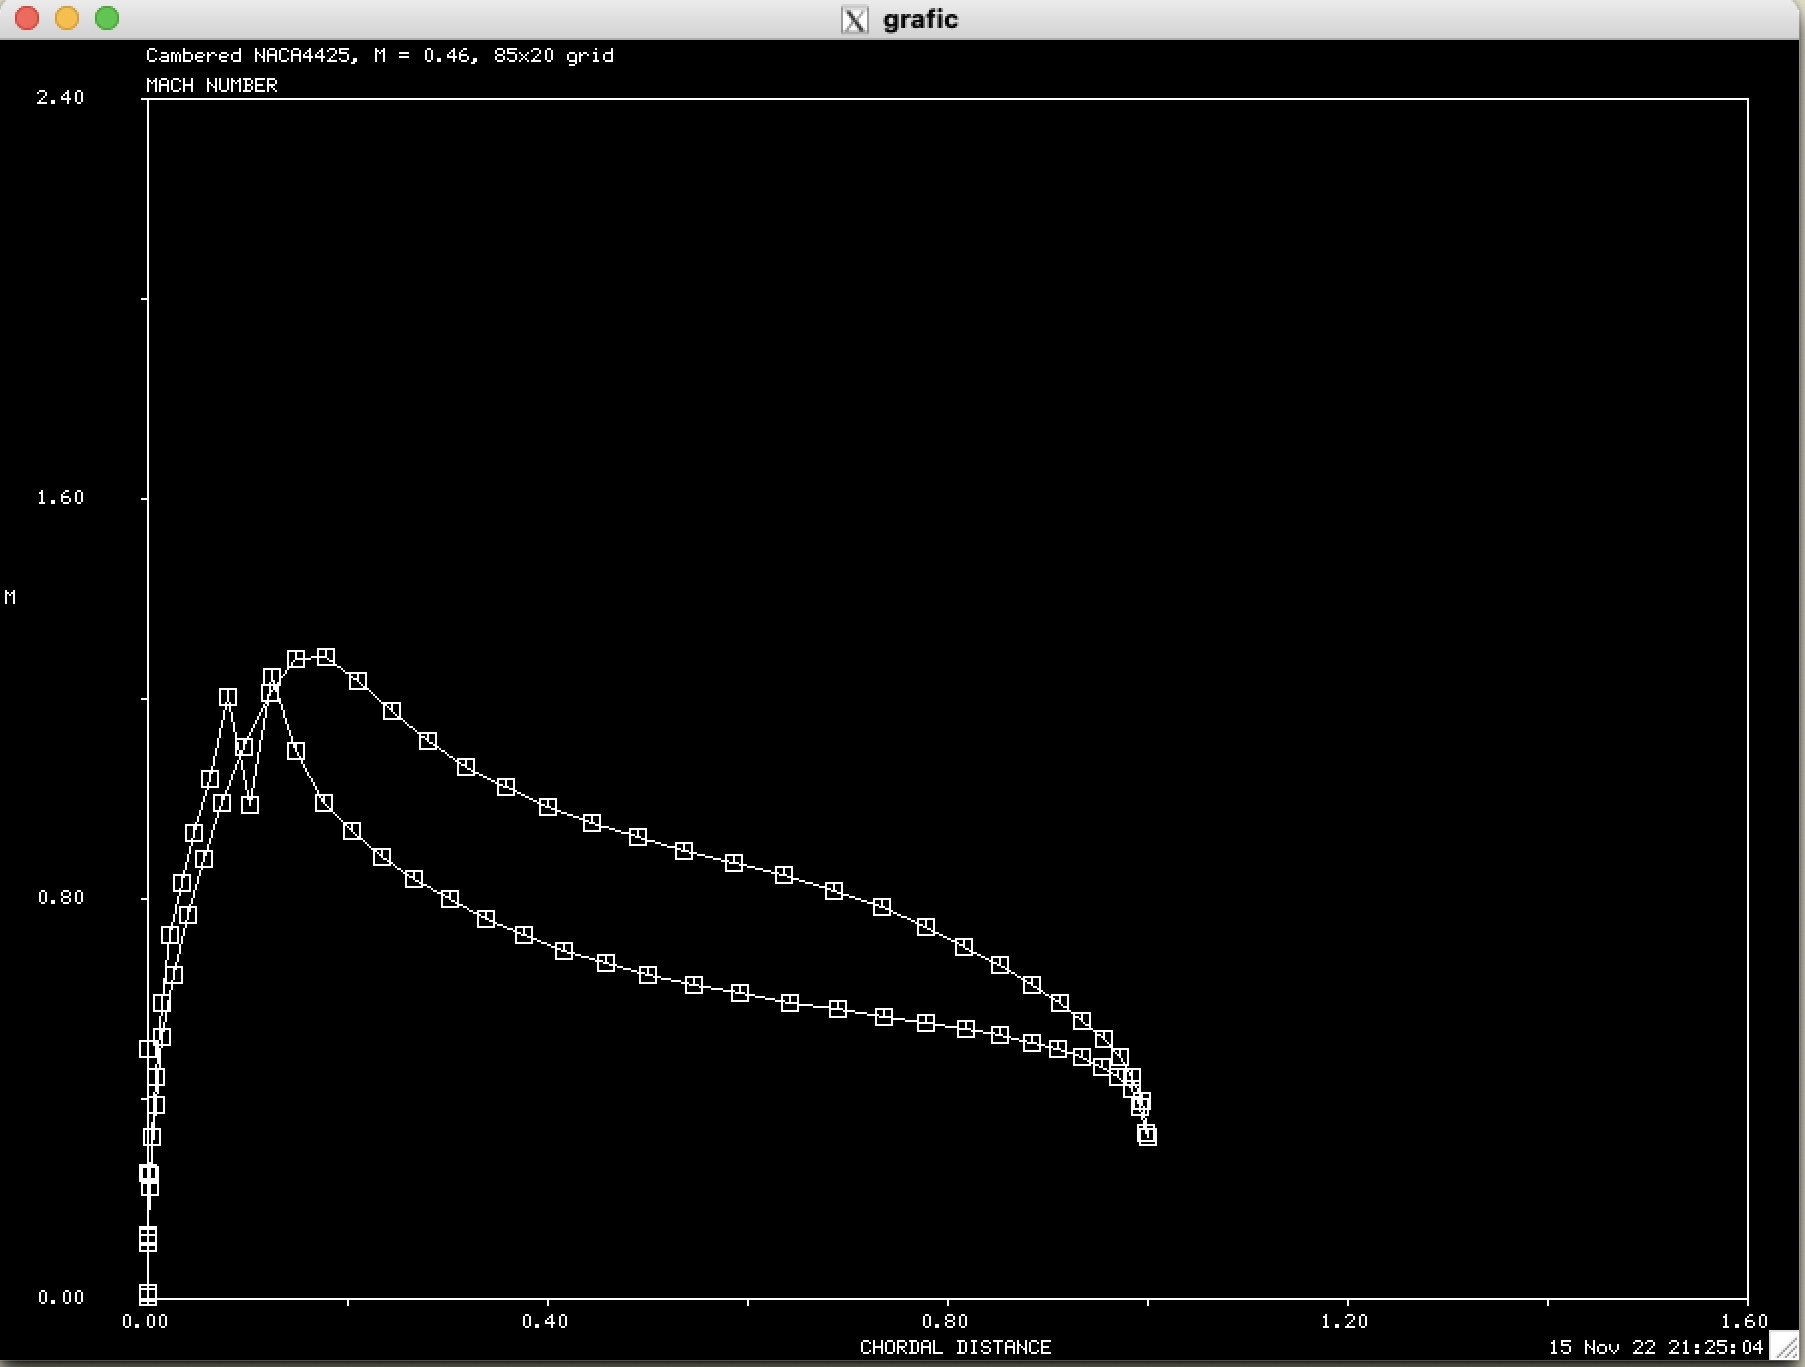
\includegraphics[width=0.75\textwidth]{/Mach.jpeg}
\end{center}

\begin{center}
  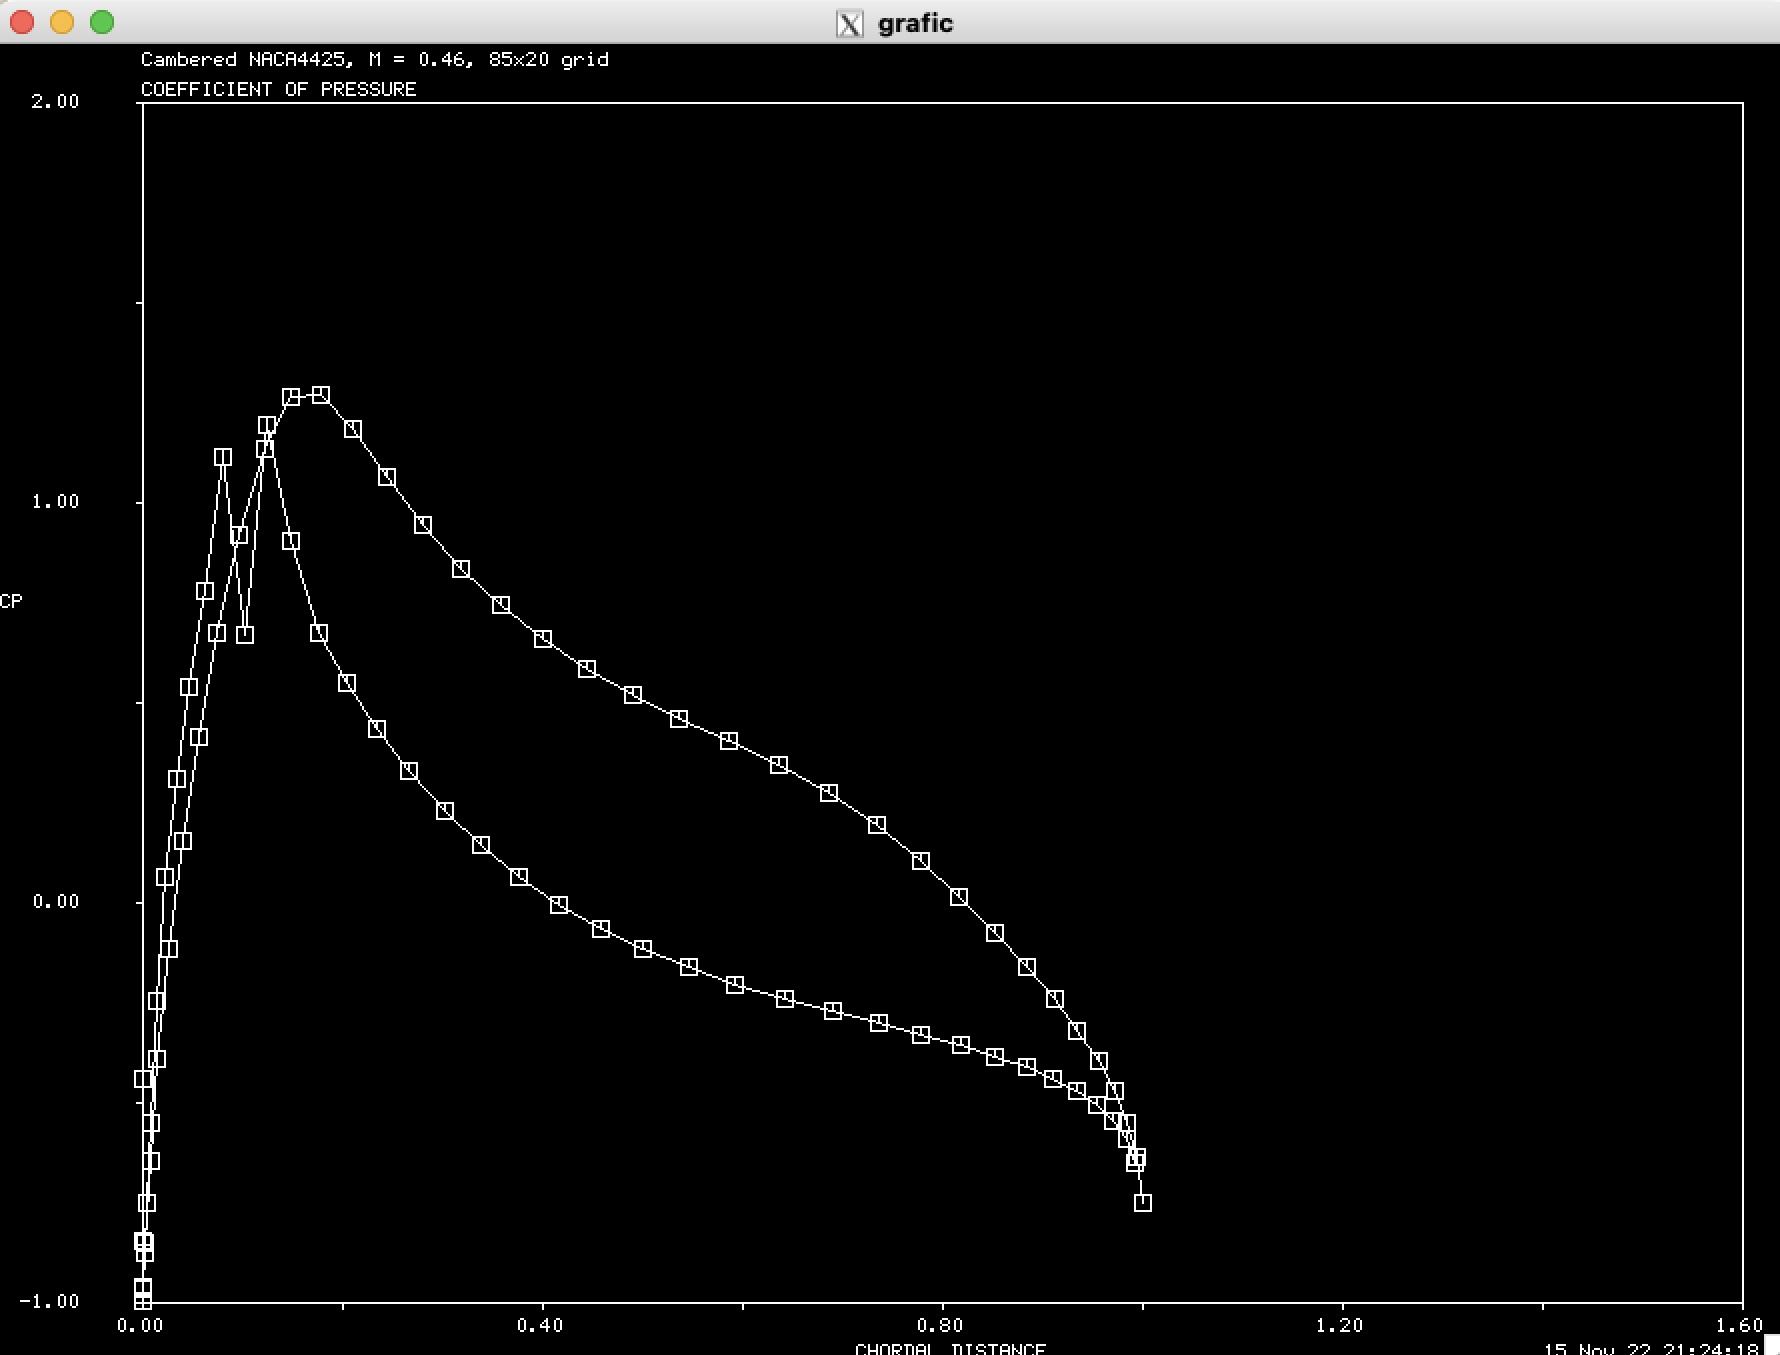
\includegraphics[width=0.75\textwidth]{/Pressure.jpeg}
\end{center}

\begin{center}
  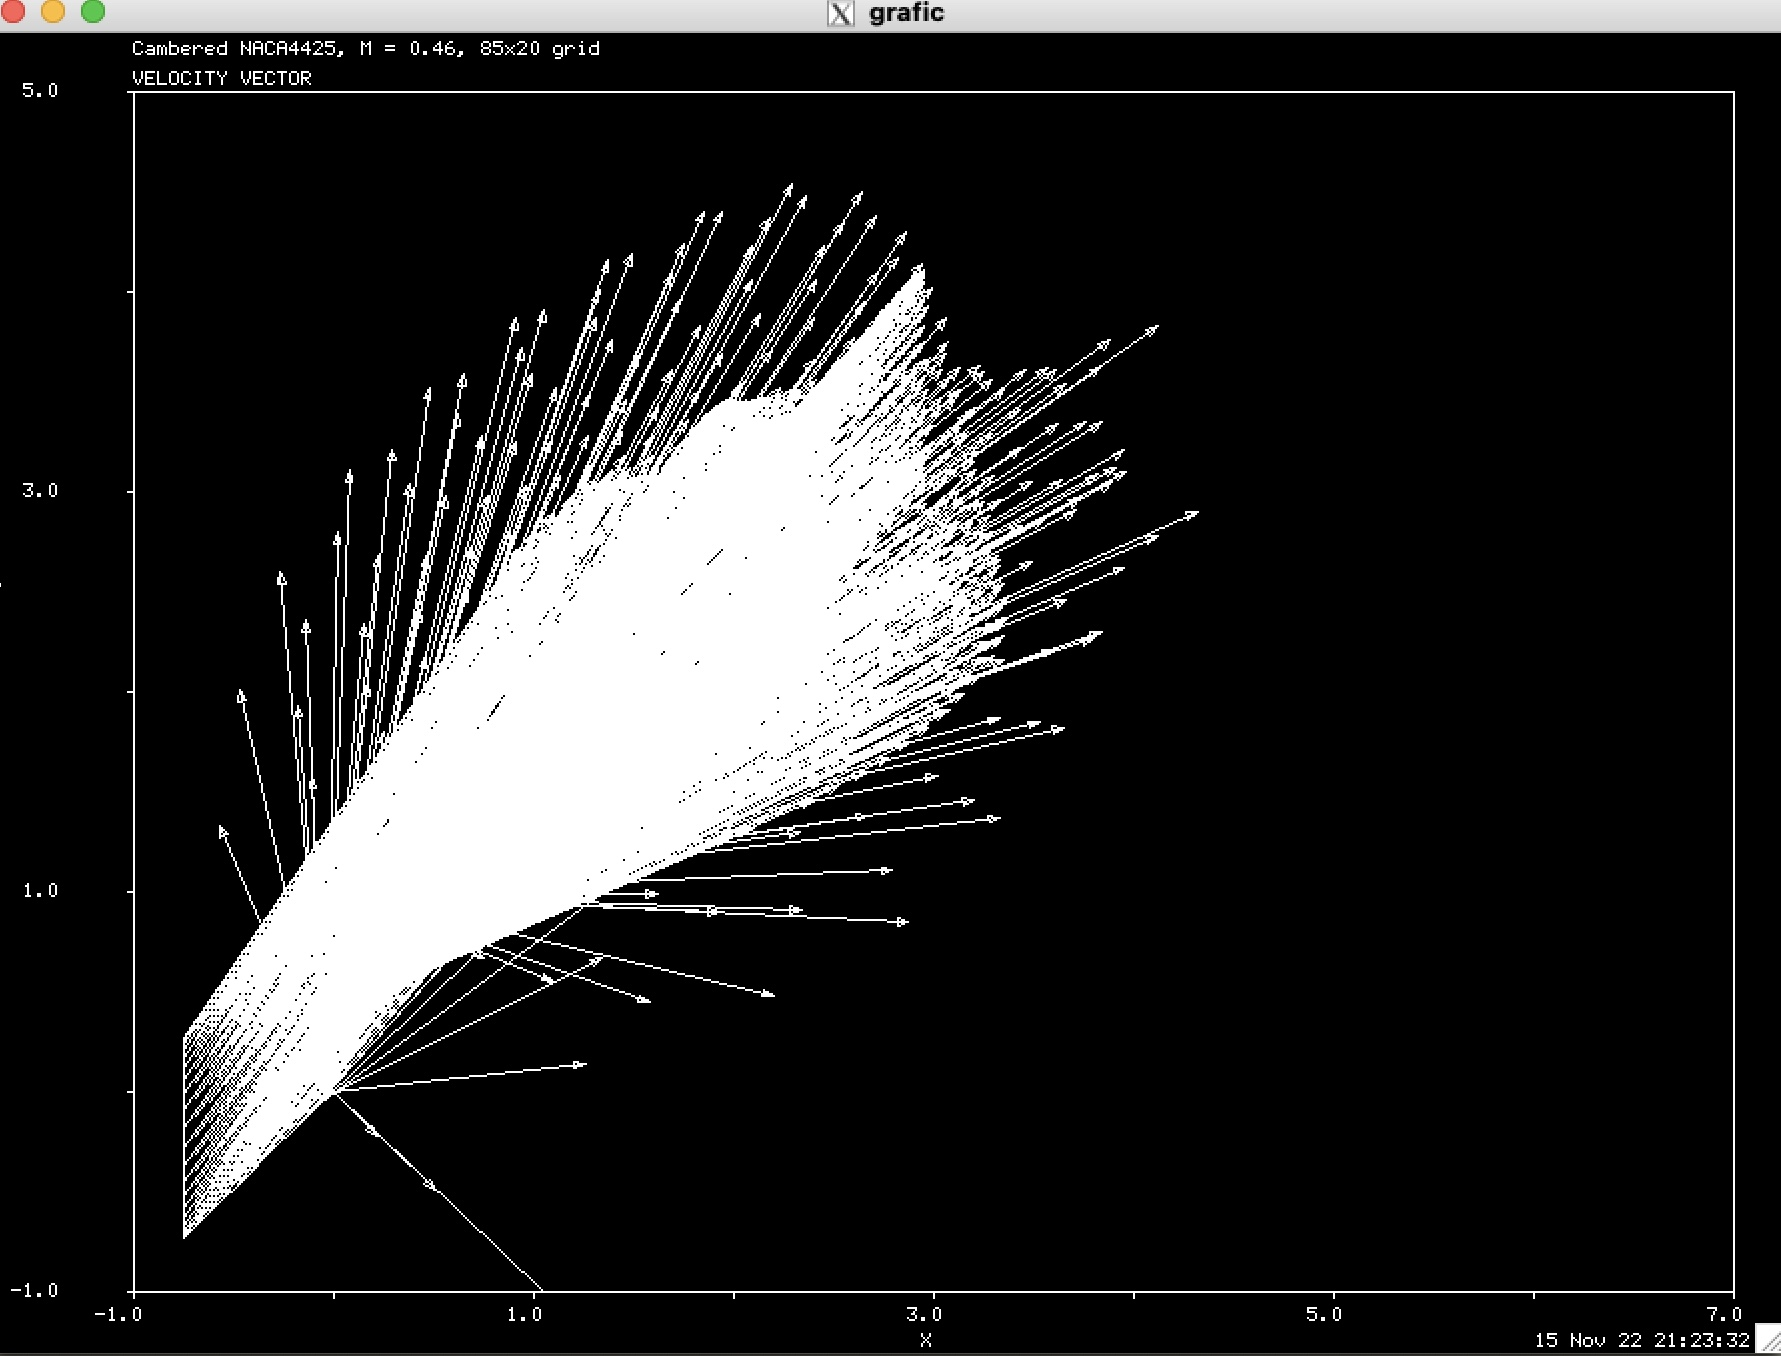
\includegraphics[width=0.75\textwidth]{/velocity.jpeg}
\end{center}




\vspace*{2cm}

\section{OLVHN - Task6}

\subsection{Overview}
This report contains the results and summary of the 12 step process described in Dr. Cizmas notes for computing the Operating Line. 
Also included in this report is the engine performance vartiatio with wheel speed, altitude and aircraft speed.

\subsection{Methodology for Computing the Operating Line}
As  we determine the Operating Line of our engine, we first define our 
operating parameters:

\begin{equation}
    \dot{m}_{air} = 1.64089 \left[\frac{kg}{s} \right]
  \end{equation}
  
  \begin{equation}
    w_{c_{n}} = 283.91025 \left[\frac{kJ}{kg}\right]
  \end{equation}
  
  \begin{equation}
    \eta_{compressor_{n}} = 0.90
  \end{equation}
  
  \begin{equation}
    \sigma_{comb} = 0.90
  \end{equation}
  
  \begin{equation}
    \eta_{turbine} = 0.94
  \end{equation}
  
  \begin{equation}
    \pi_{c_{n}} = 9.2
  \end{equation}
  
  \begin{equation}
    \lambda = 2.85377
  \end{equation}
  
  \begin{equation}
    T_{1_{n}}^{*} = 288.16 [K]
  \end{equation}
  
  \begin{equation}
    T_{3_{n}}^{*} = 1410 [K]
  \end{equation}
  
  \begin{equation}
    p_{1_{n}}^{*} =  1.01325 [bar]
  \end{equation}
  
  \begin{equation}
    p_{3_{n}}^{*} =  9.042243 [bar]
  \end{equation}
  
  \begin{equation}
    h_{3_{n}}^{*} =  1574.3477 \left[\frac{kJ}{kg}\right]
  \end{equation}
  
  \begin{equation}
    N_{n} = 52612.464822 [rpm]
  \end{equation}
  
  \begin{equation}
    \pi_{D} = 0.93
  \end{equation}
  
  \begin{equation}
    \gamma_{g} = 1.304286
  \end{equation}
  
  \begin{equation}
    \frac{A_{3.5}}{A_{5}} = 1.2
  \end{equation}
  
  \begin{equation}
    h_{1}^{*} = 288.299988 \left[\frac{kJ}{kg}\right]
  \end{equation}
  
  \begin{enumerate}
    \item Calculate the compressor work $w_{c}$, given an angular speed calculated
    in Task2, as a function of nominal compressor work and nominal angular speed.
  
    \begin{equation}
      w_{c} = w_{c_{n}} \left( \frac{N}{N_{n}} \right)^{x}
    \end{equation}
    Usually $x \in [1.9, 2.1]$, for convience we will start with $x = 2.1$.
  
    Note: 
  
    \begin{equation}
      N = 1.1N_{r}
    \end{equation}
  
    Recall when at nominal conditions:
  
    \begin{equation}
      N_{r} = \frac{N_{n}}{1.05}
    \end{equation}
  
    \begin{center}
      \begin{tabular}{|c|c|}
        \hline
        $N$ & $w_{c}$ \\
        \hline
        55117.82029 rpm & 313.0460185$\frac{kJ}{kg}$ \\
        \hline
      \end{tabular}
    \end{center}
  
    \item Estimate the compressor efficiency $\eta_{c}$, given an angular 
    speed calculated in Task2, as a function of nominal compressor efficiency and
    nominal angular speed. We start by calculated the pressure ratio $\pi_{c}^{*}$
  
    \begin{equation}
      \pi_{c}^{*} = \left[ \left(\pi_{c_{n}}^{\frac{\gamma-1}{\gamma}}\right)
      \frac{\eta_{c}}{\eta_{c_{n}}} \left(\frac{N}{N_{n}}\right)^{x} +1 \right]^{\frac{\gamma}{\gamma-1}}
    \end{equation}
  
    To begin the caluation we can start by assuming $\eta_{c} = \eta_{c_{n}}$. Once
    the pressure ratio is calculated, read that $\pi_{c}^{*}$ from the compressor map, 
    and find the corresponding $\dot{m}\frac{\sqrt{T_{1}^{*}}}{p_{1}^{*}}$. Once you have 
    that, find the corresponding $\eta_{c}$ from the compressor map. If $\eta_{c} \neq \eta_{c_{n}}$ 
    then iterate until the change is less than a allowed tolerance. For our engine,
    we allowed a tolerance of $0.01$.
  
    \begin{center}
      \begin{tabular}{|c|c|}
        \hline
        $\pi_{c}^{*}$ & $\eta_{c}$ \\
        \hline
        10.4001622 & 0.878213 \\
        \hline
      \end{tabular}
    \end{center}
    \item Calculate the $T_{3}^{*}$ from:
    
    \begin{equation}
      \pi_{c}^{*} = \frac{1+f}{\sigma_{comb}} \left( \frac{p_{3}^{*}}{\dot{m}\sqrt{T_{3}^{*}}} \right)_{n}
      \sqrt{\frac{T_{3}^{*}}{T_{1}^{*}}} \frac{\dot{m}\sqrt{T_{1}^{*}}}{p_{1}^{*}}
    \end{equation}
    Where:
    \begin{equation}
      \frac{1+f}{\sigma_{comb}} \left( \frac{p_{3}^{*}}{\dot{m}\sqrt{T_{3}^{*}}} \right)_{n} = constant
    \end{equation}
    
    From here, calculate $h_{3}^{*}$ from:
  
    \begin{equation}
      h_{3}^{*} = \left(\frac{1+minL}{1+\lambda minL}\right) h_{\lambda =1} + \left(\frac{(\lambda -1) minL}{1+\lambda minL}\right) h_{air}
    \end{equation}
  
    Where:
    \begin{itemize}
      \item $h_{\lambda}$ - enthalpy of the combustion products for $\lambda$ excess air
      \item $h_{\lambda = 1}$ - enthalpy of the combustion products for stoichiometric combustion
      \item $h_{air}$ - enthalpy of the air
    \end{itemize}
  
    Check to see if the ratio $\frac{w_{c}}{h_{3}^{*}}$ is equal to the nominal ratio
    $\frac{w_{c_{n}}}{h_{3_{n}}^{*}}$. If not, iterate x until it is, within a reasonable tolerance of about 1\%.
  
    \vspace{0.5cm}
  
    After iterating x, we arrived to $x = 1.4$.
  
    \begin{center}
      \begin{tabular}{|c|c|}
        \hline
        $T_{3}^{*}$ & $h_{3}^{*}$ \\
        \hline
        1552.103717 [K] & 1753.74986 $\frac{kJ}{kg}$ \\
        \hline
      \end{tabular}
    \end{center}
  
    \item We are now to find the critical conditions by:
    
    \begin{equation}
      \pi_{c_{cr}}^{*} = \frac{1}{\sigma_{comb} \pi_{D}} \left[ \frac{\frac{\gamma_{g}+1}{2}}{1 - \frac{w_{c}}{h_{3}^{*}} \frac{1}{\eta_{turbine}}} \right]^{\frac{\gamma_{g}}{\gamma_{g}-1}}
    \end{equation}
  
    \begin{equation}
      N_{cr} = N_{n} \sqrt{\frac{\eta_{c_{n}}}{\eta_{c_{cr}}}} \frac{\pi_{c_{cr}}^{\frac{\gamma - 1}{\gamma}} -1}{\pi_{c_{n}}^{\frac{\gamma -1}{\gamma}} - 1}
    \end{equation}
  
    We are to then repeat steps (1)-(3) for three values of angular speed
    larger than the critical angular speed.
  
    \begin{center}
      \begin{tabular}{|c|c|c|}
        \hline
        $\pi_{c_{cr}}^{*}$ & $N_{cr}$ & $\eta_{c_{cr}}$ \\
        \hline
        5.462985 & 44711.24058 rpm & 0.879 \\
        \hline
      \end{tabular}
    \end{center}
  
    \begin{center}
      \begin{tabular}{|c|c|c|}
        \hline
        $\frac{w_{c}}{h_{3}^{*}}$ & $\left(\frac{w_{c}}{h_{3}^{*}}\right)_{n}$ & \% diff \\
        \hline
        0.1785009519 & 0.180335162 & 1.0171116 \% \\
        \hline
      \end{tabular}
    \end{center}
  
    Now we repeat steps (1)-(3) for three values of angular speed larger than the critical angular speed.
  
    \begin{center}
      \begin{tabular}{|c|c|c|c|c|c|c|c|c|}
        \hline
        $N$ & $w_{c}$ & $\eta_{iteration}$ & $\pi_{c}^{*}$ & $\bar{m}$ \\
        \hline
        46946.803 & 223.4949 & 0.881 & 6.17351 & 0.71 \\
        \hline
        49182.365 & 246.4306 & 0.879 & 7.09622 & 0.785 \\
        \hline
        51417.93	& 270.5425 & 0.9	& 8.5075	& 0.9 \\
        \hline
      \end{tabular}
    \end{center}
  
    \begin{center}
      \begin{tabular}{|c|c|c|c|c|}
        \hline
        $N$ & $T_{3}^{*}$ & $h_{3}^{*}$ & $\frac{w_{c}}{h_{3}^{*}}$ & \% diff \\
        \hline
        46946.803 & 1150.965 & 1251.825 & 0.17854 & 0.998 \\
        \hline
        49182.365 & 1244.026485 & 1368.077 &	0.18013	& 0.1142 \\
        \hline
        51417.93 & 1360.3106 & 1512.1349	& 0.1789	& 0.7879 \\
        \hline
      \end{tabular}
    \end{center}
  
  
    \item Once we have reached the critical value, our ratio $\frac{w_{c}}{h_{3}^{*}}$ is no longer constant. If the flow isn't critical,
    then the variation of $\frac{w_{c}}{h_{3}^{*}}$ is given by:
  
    \begin{equation}
      \frac{w_{c}}{h_{3}^{*}} = \eta_{turbine} \left[ 1 - \left(\frac{p_{H}}{p_{3}^{*}}\right)^{\frac{\gamma_{g}-1}{\gamma_{g}}} - K \left(\frac{A_{3.5}}{A_{5}}\right)^{2} \left(\frac{p_{3}^{*}}{p_{H}}\right)^{\frac{2}{\gamma_{g}}} \right] 
    \end{equation}
    
    Where:
  
    \begin{equation}
      K = \left(\frac{A_{5}}{A_{3.5}}\right)^{2} \left(\frac{p_{H}}{p_{3}^{*}}\right)^{\frac{2}{\gamma_{g}}}\left[1 - \left(\frac{p_{H}}{p_{3}^{*}}\right)^{\frac{\gamma_{g}-1}{\gamma_{g}}} \frac{w_{c}}{h_{3}^{*}} \frac{1}{\eta_{turbine}}\right] 
    \end{equation}
  
    \begin{equation}
      \frac{p_{H}}{p_{3}^{*}} = \frac{1}{\sigma_{combustion}^{*} \pi_{c}^{*} \pi_{D}}
    \end{equation}
  
    Recall that $\pi_{D}$ is given by:
  
    \begin{equation}
      \pi_{D} = \frac{p_{1}^{*}}{p_{H}}
    \end{equation}
  
    When performing this step be sure to choose a $\pi_{c}^{*}$ that is less than the critical value $\pi_{c_{cr}}^{*}$.
  
    \begin{center}
      \begin{tabular}{|c|c|c|}
        \hline
        $K$ & $\frac{p_{H}}{p_{3}^{*}}$ & $\frac{w_{c}}{h_{3}^{*}}$ \\
        \hline
        0.007177101 & 0.23020826 & 0.180335162\\
        \hline
      \end{tabular}
    \end{center}
  
    \item Now we are to choose an $N$ value smaller than the critical value $N_{cr}$, and calculate $w_{c}$ using equation (16)
    We chose a $N$ value that was 1\% less than the critical value.
  
    \begin{equation}
      N < N_{cr}
    \end{equation}
  
    Now we use equation (16) to calculate $w_{c}$. 
  
    \begin{center}
      \begin{tabular}{|c|c|}
        \hline
        $N$ & $w_{c}$ \\
        \hline
        44500 rpm & 199.73351054474077 $\frac{kJ}{kg}$ \\
        \hline
      \end{tabular}
    \end{center}
  
    \item Now calculate $h_{3}^{*}$ from equation (26) and $w_{c} = 171.430154 \frac{kJ}{kg}$.
    
    \begin{equation}
      h_{3}^{*} = w_{c_{n}} \left( \frac{w_{c}}{h_{3}^{*}}\right)^{-1}
    \end{equation}
  
    \begin{center}
      \begin{tabular}{|c|}
        \hline
        $h_{3}^{*}$ \\
        \hline
        1107.56831 $\frac{kJ}{kg}$ \\
        \hline
      \end{tabular}
    \end{center}
  
    \item Calculate $T_{3}^{*}$ using the stoichiometric and air gas tables. 
    
    \begin{center}
      \begin{tabular}{|c|}
        \hline
        $T_{3}^{*}$ \\
        \hline
        1028.878066 K \\
        \hline
      \end{tabular}
    \end{center}
  
    \item For known value of $\pi_{c}^{*}$ and $N$ read from the the compressor map the value of the corrected mass flow rate
  
    \begin{equation}
      \pi{_c}^{*} = 5.18983611172067
    \end{equation}
  
    Yields a corrected mass flow rate of:
  
    \begin{center}
      \begin{tabular}{|c|}
        \hline
        $m_{a}\frac{\sqrt{T_{1}^{*}}}{p_{1}^{*}}$ \\
        \hline
        (0.63)(1.6087157)$\frac{\sqrt{288}}{101325}$ \\
        \hline
      \end{tabular}
    \end{center}
  
    \item Now determine $T_{3}^{*}$ using equation (21).
    \item Compare the values of $T_{3}^{*}$ from step 8 to $T_{3}^{*}$ from step 10, if they differ by more than 10 degrees K, then iterate until with different $N$ value.
    
    \begin{center}
      \begin{tabular}{|c|}
        \hline
        $T_{3}^{*}$ \\
        \hline
        1033.097120243129 K \\
        \hline
      \end{tabular}
    \end{center}
  
  \item Now choose another value of $\pi_{c}^{*}$ and go back to step 5 and repeat the process to get other points on the operating line at $\frac{p_{H}}{p_{3}^{*}}$ 
  
  \begin{center}
    \begin{tabular}{|c|c|c|c|c|c|}
      \hline
      $\pi_{c}^{*}$ & $\frac{p_{H}}{p_{3}^{*}}$ & $K$ & $\frac{w_{c}}{h_{3}^{*}}$ & $N$ \\
      \hline
      6.009283919	& 0.198816223	& 0.007124393 &	0.180335162	& 44500 \\
      \hline
      7.101880995	& 0.168229112 &	0.006698233 &	0.180335162	& 40000 \\
      \hline
      8.194478071 &	0.145798563 &	0.006163854	& 0.180335162	& 50000 \\
      \hline
    \end{tabular}
  \end{center}
  
  \begin{center}
    \begin{tabular}{|c|c|c|c|}
      \hline
      $w_{c}$ & $h_{3}^{*}$ & $T_{3}^{*}$ & $T_{3}^{*}$ \\
      \hline
      199.73351054474077	& 1107.56831	& 1028.878066	& 1033.097120243129 \\
      \hline
      159.6691061	& 885.4019626 &	839.0287095 & 833.1424783 \\
      \hline
      255.1126073	& 1414.658156	& 1281.631036 & 1276.178685 \\
      \hline
    \end{tabular}
  \end{center}
  
  
  
  \end{enumerate}
  
  \begin{center}
    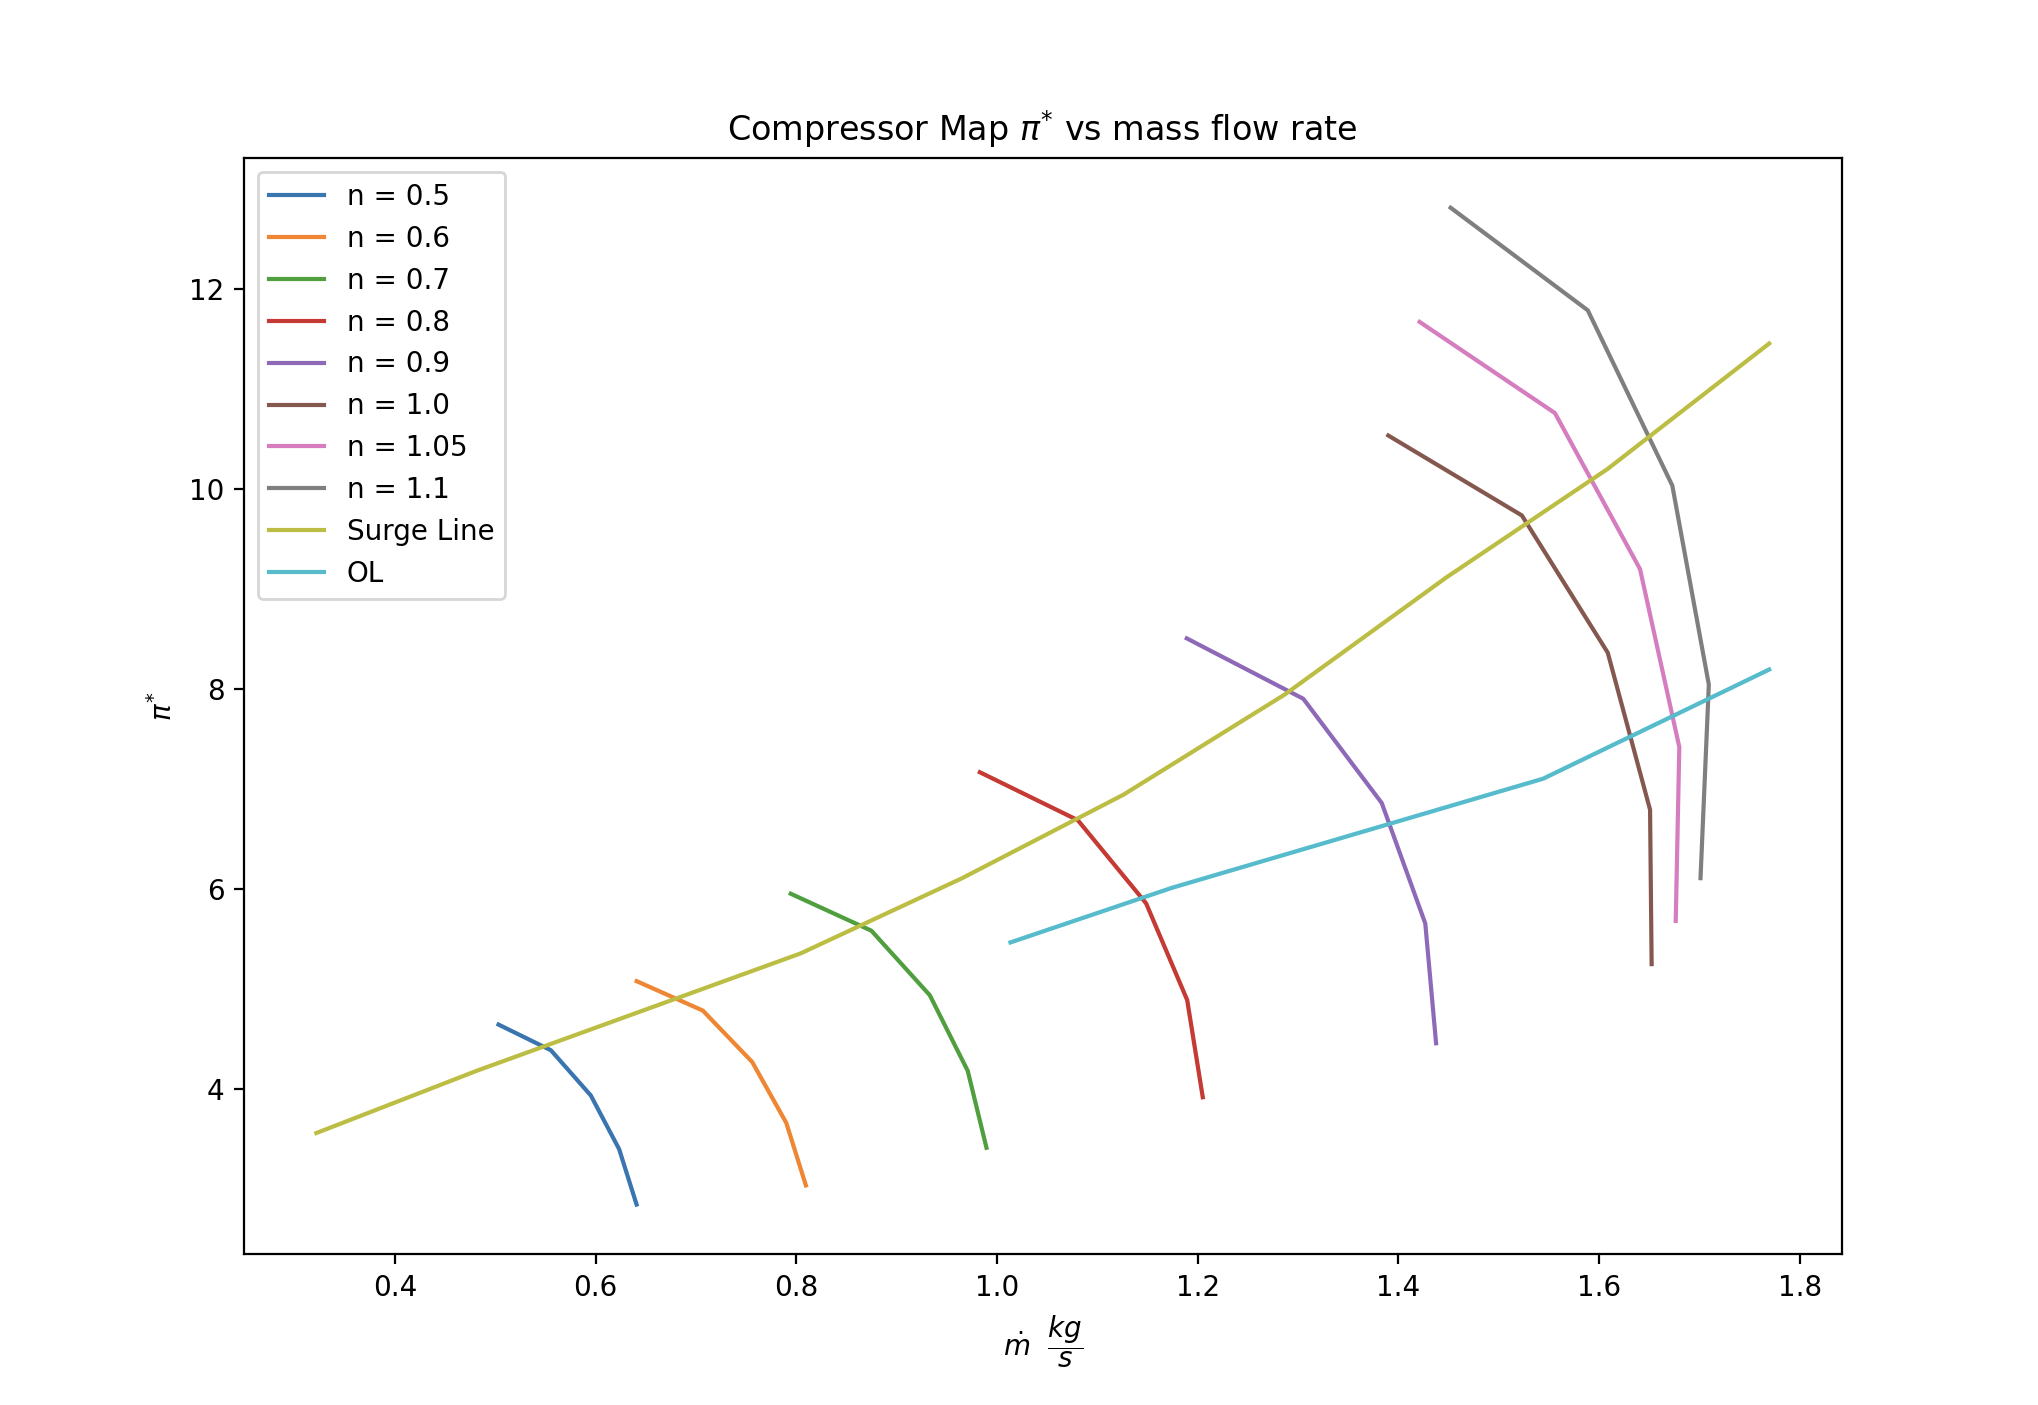
\includegraphics[width=\textwidth]{CompressorMap.png}
  \end{center}
  
  \vspace{2cm}

  \subsection{Jet Engine Performance Variation with Wheel Speed}

  To determine the performance variation with wheel speed (N) we are to use the \textbf{Operating Line} from Section 2. We will choose wheel speeds that are different 
from the nominal wheel speed $N_{n}$, and then read from the Compressor Map the pressure ratios $\pi_{c}^{*}$ and the efficiencies $\eta_{c}$.

\begin{center}
  \begin{tabular}{|c|c|c|}
    \hline
    $N$ & $\pi_{c}^{*}$ & $\eta_{c}$ \\
    \hline
    40000 rpm & 7.101880995 & 0.849 \\
    \hline
    44500 rpm & 6.009283919 & 0.877 \\
    \hline
    49000 rpm & 7.9900312 & 0.8325 \\
    \hline
  \end{tabular}
\end{center}

Now similar to how we solved for compressor work, we make use of equation (17):

\begin{center}
  $$w_{c} = w_{c_{n}} \left( \frac{N}{N_{n}}\right)^{x}$$
\end{center}

Here we will use $x = 2$ following Dr. Cizmas' Example.

\begin{center}
  \begin{tabular}{|c|}
    \hline
    $w_{c}$ \\
    \hline
    203.1064891\\
    \hline
    164.1057354 \\
    \hline
    246.2611692 \\
    \hline
  \end{tabular}
\end{center}

The enthalpy at stage 02 is calculated:

\begin{equation}
  h_{2}^{*} = h_{1}^{*} + w_{c}
\end{equation}

\begin{center}
  \begin{tabular}{|c|}
    \hline
    $h_{2}^{*}$ \\
    \hline
    491.4064771 \\
    \hline
    452.4057234 \\
    \hline
    534.5611572 \\
    \hline
  \end{tabular}
\end{center}

The degree of dynamic compression in the inlet nozzle is recalculated as:

\begin{equation}
  \pi_{D} = \sigma_{inlet}^{*} \left( 1+\frac{\gamma - 1}{2}M_{H}^{2}\right)^{\frac{\gamma}{\gamma - 1}}
\end{equation}

Recall $\sigma_{inlet}^{*} = 0.93$. Also here we are assuming $M_{H} = 0$, since we are at Take-off conditions.

\begin{center}
  \begin{tabular}{|c|}
    \hline
    $\pi_{D}$ \\
    \hline
    0.93 \\
    \hline
    0.93 \\
    \hline
    0.93 \\
    \hline
  \end{tabular}
\end{center}

The specific thrust is now recalculated as:

\begin{equation}
  F_{sp} = \phi \sqrt{2h_{3}^{*}\left[1 - \frac{1}{\pi_{D} \pi_{c}^{*} \sigma_{comb}^{*}}\right]^{\frac{\gamma_{g}-1}{\gamma_{g}}} - h_{1}^{*}\left(\frac{\pi_{c}^{\frac{\gamma-1}{\gamma}}}{\eta_{c}}\right)} \left(1+\frac{1}{\lambda minL}\right)
\end{equation}

\begin{center}
  \begin{tabular}{|c|c|c|c|c|}
    \hline
    $F_{sp}$ & $\frac{p_{H}}{p_{3}^{*}}$ & $K$ & $\frac{w_{c}}{h_{3}^{*}}$ & $h_{3}^{*}$ \\
    \hline
    731.102889 & 0.198816223	& 0.007124393 &	0.180335162	& 1126.272254 \\
    \hline
    656.888117 & 0.168229112	& 0.006698233	& 0.180335162	& 910.0040937 \\
    \hline
    875.895256 & 0.149529804 & 0.006265198	& 0.180335162	& 1365.574893 \\
    \hline
  \end{tabular}
\end{center}

The mass flow rate is recalculated as:

\begin{equation}
  \dot{m}_{air} = \dot{m}_{air_{n}} \frac{\pi{c}^{*}}{\pi_{c_{n}}^{*}} \frac{N_{n}}{N}
\end{equation}

\begin{center}
  \begin{tabular}{|c|}
    \hline
    $\dot{m}_{air}$ \\
    \hline
    1.26719369 \\
    \hline
    1.666071704 \\
    \hline
    1.530139367 \\
    \hline
  \end{tabular}
\end{center}

And the TSFC is recalculated as:

\begin{equation}
  TSFC = \frac{3600}{F_{sp}} \frac{1}{\lambda minL}
\end{equation}

\begin{center}
  \begin{tabular}{|c|}
    \hline
    TSFC \\
    \hline
    0.117699 \\
    \hline
    0.130996 \\
    \hline
    0.098242 \\
    \hline
  \end{tabular}
\end{center}

\begin{center}
    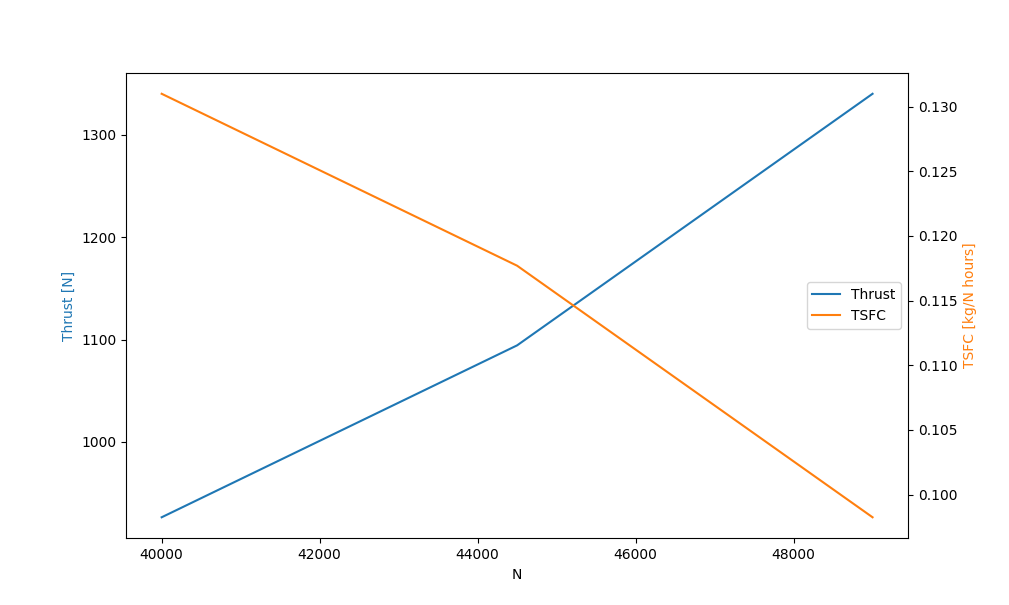
\includegraphics[width=\textwidth]{fig_N.png}
\end{center}

Above is the the plot of the engine performance variation with wheel speed $N$ [rpm]

\subsection{Jet Engine Performance Variation with Altitude and Speed}

Up to this point, our engine has been performance has been calculate at take-off conditions. It is very important for us to determine how the 
performance varies with altitude and speed. 

\begin{enumerate}
  \item First we are to calculate the Mach number at H and V.
  
  \begin{equation}
    M_{H} = \frac{V}{\sqrt{\gamma R T_{H}}}
  \end{equation}

  It is important for us to specify our altitude dependent properties and speed dependent properties.

  \begin{center}
    \begin{tabular}{|c|c|c|c|}
      \hline
      $H$ [m] & $T_{H}$ [K] & $p_{H}$ [Pa] & $a_{H}$ [m/s] \\
      \hline
      0 & 288.15 & 101325 & 340.29 \\
      \hline
      1000 & 281.65 & 89874.6	& 336.434 \\
      \hline
      3000	& 268.65	& 70108.5	& 328.578 \\
      \hline
      5000	& 255.65	& 54019.9	& 320.529 \\
      \hline
      6000	& 249.15	& 47181 &	316.428 \\
      \hline
      7000 &	242.65	& 41060.7	& 312.274 \\
      \hline
      8000	& 236.15	& 35599.8	& 308.063 \\
      \hline
      9000	& 229.65	& 30742.5 &	303.793 \\
      \hline
      10000	& 223.15	& 26436	& 299.463 \\
      \hline
    \end{tabular}
  \end{center}

  And our velocity values:

  \begin{center}
    \begin{tabular}{|c|}
      \hline
      $v$ [m/s] \\
      \hline
      0 \\
      \hline
      100 \\
      \hline
      200 \\
      \hline
      300 \\
      \hline
      350 \\
      \hline
      400 \\
      \hline
    \end{tabular}
  \end{center}

  \item Now one can calculate the degree of dynamic compression $\pi_{D}$.
   \begin{equation}
      \pi_{D} = \frac{p_{1}^{*}}{p_{H}} = \sigma_{inlet}^{*} \frac{p_{H}^{*}}{p_{H}}
   \end{equation}


   This means that we can say:
   \begin{equation}
    \pi_{D} = \sigma_{inlet}^{*} \left(1+\frac{\gamma-1}{2} M_{H}^{2}\right)^{\frac{\gamma}{\gamma-1}}
   \end{equation}

   Where $\sigma_{inlet}^{*}$ is the inlet stagnation pressure loss in the inlet defined as the ratio between the stagnation pressure at the inlet
   in the compressor $p_{1}^{*}$ and the stagnation pressure at the inlet of the engine $p_{H}$.

   \begin{center}
    \begin{tabular}{c c c c c c c c c c c }
      \hline
      \textbf{$H$ [km]} & 0 & 1 & 3 & 5 & 6 & 7 & 8 & 9 & 1 & \textbf{$v$ [m/s]} \\
      \hline
      \textbf{$\pi_{D}$} & 0.93 &	0.93	& 0.93	& 0.93	& 0.93 &	0.93 & 	0.93 & 	0.93 & 	0.93 & 0 \\
      \hline
      \textbf{$\pi_{D}$} & 0.9889	& 0.9887	& 0.9917 & 	0.9949	& 0.9966	& 0.9985	& 1.0004 & 	1.0024 &	1.0046 & 100 \\
      \hline
      \textbf{$\pi_{D}$} & 1.1809	&1.1810	&1.1943	& 1.2090	&1.2170	& 1.2254 &	1.2344 &	1.2439 &	1.2541 & 200 \\
      \hline
      \textbf{$\pi_{D}$} &1.5566&	1.5586	&1.5952	&1.6361&	1.6585	&1.6823	&1.7077	&1.7348	&1.7638& 300 \\
      \hline
      \textbf{$\pi_{D}$} &1.8411	&1.8460	&1.9023	&1.9656	&2.0004	&2.0375	&2.0772	&2.1197	&2.1654& 350 \\
      \hline
      \textbf{$\pi_{D}$} &2.2122	&2.2226	&2.3066	&2.4019&	2.4544	&2.5105	&2.5708	&2.6356	& 2.7054& 400 \\
      \hline
    \end{tabular}
  \end{center}

  \item Now we calculate $h_{H}^{*}$.
   \begin{equation}
    h_{H}^{*} = h_{H}\left( 1+ \frac{\gamma-1}{2} M_{H}^{2} \right)
   \end{equation}  

   \item Now calculate the compressor pressure ratio $\pi_{c}^{*}$ with variation of H and V.
   
   \begin{equation}
    \pi_{c}^{*} = \left[ 1+ \frac{h_{0}}{h_{H}^{*}}\left(\pi_{c_{n}}^{* \frac{\gamma-1}{\gamma}} - 1\right) \right] ^{\frac{\gamma}{\gamma-1}}
   \end{equation}

   Students can also calculate $w_{c}$:

   \begin{equation}
    w_{c} = h_{2}^{*} - h_{H}^{*}
   \end{equation}

   \item Now oen can begin calculating the Specific Thrust $F_{sp}$
   \begin{equation}
    F_{sp} = \phi_{5} \sqrt{2h_{3}^{*}\left[1-\frac{1}{(\pi_{D} \pi_{c}^{*} \pi_{combust}^{*})} \right] - h_{1}^{*}}\frac{\pi_{c}^{\frac{\gamma-1}{\gamma}}}{\eta_{c}}\left(1+\frac{1}{\lambda minL}\right) - v
    \end{equation}

  Recall, $\gamma$ varies due to the variance in speed of sound $a$ from the change in altitude.
  
  \begin{equation}
    \gamma = \frac{a_{H}^{2}}{R_{air}T_{H}}
  \end{equation}

  We can calculate $h_{3}^{*}$ similar to previous sections:

  \begin{equation}
    h_{3}^{*} = \left(\frac{w_{c}}{h_{3}^{*}}\right) w_{c}
  \end{equation}
  
  Where $w_{c}$ comes from equation (44) and $\frac{w_{c}}{h_{3}^{*}}$ comes from equations (27), (28), and (29).

  \begin{center}
  
    $\frac{w_{c}}{h_{3}^{*}} = \eta_{turbine} \left[ 1 - \left(\frac{p_{H}}{p_{3}^{*}}\right)^{\frac{\gamma_{g}-1}{\gamma_{g}}} - K \left(\frac{A_{3.5}}{A_{5}}\right)^{2} \left(\frac{p_{3}^{*}}{p_{H}}\right)^{\frac{2}{\gamma_{g}}} \right] $


    $K = \left(\frac{A_{5}}{A_{3.5}}\right)^{2} \left(\frac{p_{H}}{p_{3}^{*}}\right)^{\frac{2}{\gamma_{g}}}\left[1 - \left(\frac{p_{H}}{p_{3}^{*}}\right)^{\frac{\gamma_{g}-1}{\gamma_{g}}} \frac{w_{c}}{h_{3}^{*}} \frac{1}{\eta_{turbine}}\right] $


    $\frac{p_{H}}{p_{3}^{*}} = \frac{1}{\sigma_{combustion}^{*} \pi_{c}^{*} \pi_{D}}$
  \end{center}
  
Now all we have to solve for is the varying $\lambda$. We begin by making use of the energy conservation equation between the inlet and burner.

\begin{equation}
  \dot{m}_{air}h_{2}^{*} + \dot{m}_{fuel} \left(h_{fuel} + \pi_{combust}^{*}LHV\right) = \dot{m}_{air}h_{3}^{*} 
\end{equation}

Recall $LHV = 43.5 \times 10^{6} J/kg$ for standard fuel. We can make use of:

\begin{equation}
  f = \frac{\dot{m}_{fuel}}{\dot{m}_{air}} = \frac{1}{L} = \frac{1}{\lambda minL}
\end{equation}

Resulting in the following equation:

\begin{equation}
  h_{2}^{*} + \frac{\pi_{combust}^{*} LHV}{\lambda minL} = \left[1+ \frac{1}{\lambda minL}\right] h_{3}^{*}
\end{equation}

We have all the necessary variables to solve for $\lambda$, therfore equation (45) can be solved.

\begin{center}
  \begin{tabular}{c c c c c c c c c c c }
    \hline
    \textbf{$H$ [km]} & 0 & 1 & 3 & 5 & 6 & 7 & 8 & 9 & 1 & \textbf{$v$ [m/s]} \\
    \hline
    $F_{sp}$ & 1040	&1002.6	&1032	&1060.84	&1075.03	&1089.1	&1103	&1116.8	&1130.5 & 0 \\
    \hline
    $F_{sp}$ & 938.35	&900.6&	930.9	&960.5	&975.2	&989.6	&1004.01	&1018.3	&1032.5& 100 \\
    \hline
    $F_{sp}$ & 830.5	&792.0	&824.4	&856.4	&872.2	&888.0	&903.7	&919.3	&934.8& 200 \\
    \hline
    $F_{sp}$ & 709.5	&669.3	&705.2	&740.7	&758.3	&775.9	&793.4	&810.9	&828.3& 300 \\
    \hline
    $F_{sp}$ & 641.0	&599.4	&637.4	&675.0	& 693.7	&712.3	&730.8	&749.4	&767.9& 350 \\
    \hline
    $F_{sp}$ & 565.0	&521.5	&562.0	&601.9	&621.7	&641.5	&661.2	&680.9	&700.6& 400 \\
    \hline
  \end{tabular}
\end{center}

One can now calculate $TSFC$:

\begin{equation}
  TSFC = (TSFC)_{n} \frac{F_{sp_{n}}}{F_{sp}} \frac{\lambda_{n}}{\lambda}
\end{equation}



\begin{center}
  \begin{tabular}{c c c c c c c c c c c }
    \hline
    \textbf{$H$ [km]} & 0 & 1 & 3 & 5 & 6 & 7 & 8 & 9 & 1 & \textbf{$v$ [m/s]} \\
    \hline
    $TSFC$ &0.1037	&0.0985	&0.1026	&0.1066	&0.1085	&0.1104	&0.1123	&0.1142	&0.1160& 0 \\
    \hline
    $TSFC$ &0.1120	&0.1066	&0.1108	&0.1149	&0.1168	&0.1187	&0.1206	&0.1225	&0.1243& 100 \\
    \hline
    $TSFC$ &0.1167	&0.1109	&0.1152	&0.1192	&0.1211	&0.1230	&0.1249	&0.1267	&0.1284& 200 \\
    \hline
    $TSFC$ &0.1174	&0.1110	&0.1154	&0.1194	&0.1213	&0.1232	&0.1250	&0.1267	&0.1283& 300 \\
    \hline
    $TSFC$ &0.1163&	0.1094	&0.1139	&0.1180	&0.1199	&0.1218	&0.1235	&0.1252	&0.1268& 350 \\
    \hline
    $TSFC$ &0.1140	&0.1066	&0.1112	&0.1154	&0.1173	&0.1192	&0.1209	&0.1225	&0.1240& 400 \\
    \hline
  \end{tabular}
\end{center}

One can calculate mass flow rate by:

\begin{equation}
  \dot{m_{a}} = \dot{m}_{a_{n}} \frac{\pi_{c}^{*}}{\pi_{c_{n}}^{*}} \frac{p_{H}}{p_{0}} \left( 1+ \frac{\gamma-1}{2}M_{H}^{2}\right)^{\frac{\gamma}{\gamma-1}} \frac{\sigma_{inlet}^{*}}{\sigma_{inlet_{n}}^{*}}
\end{equation}

\item Finally calculate Thrust:

\begin{equation}
  F = F_{sp} \dot{m_{a}}
\end{equation}

\end{enumerate}

\begin{center}
    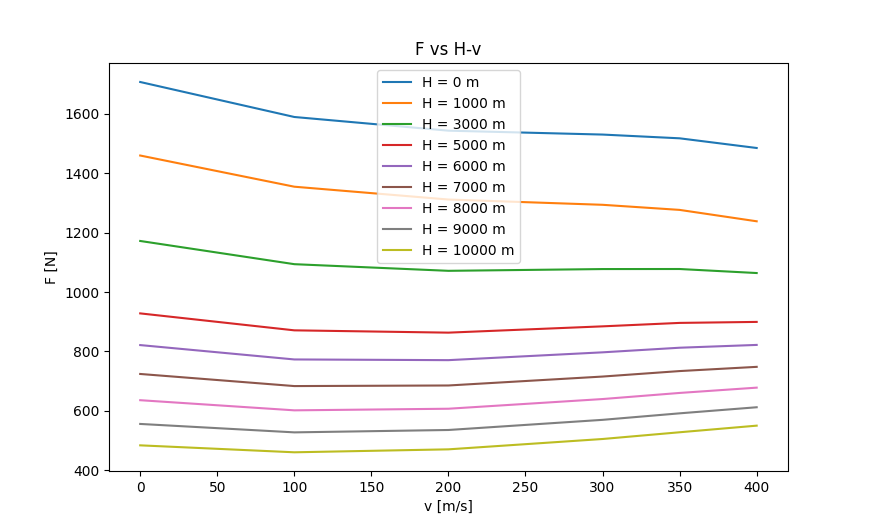
\includegraphics[width=\textwidth]{FHV.png}
\end{center}
  
  \begin{center}
    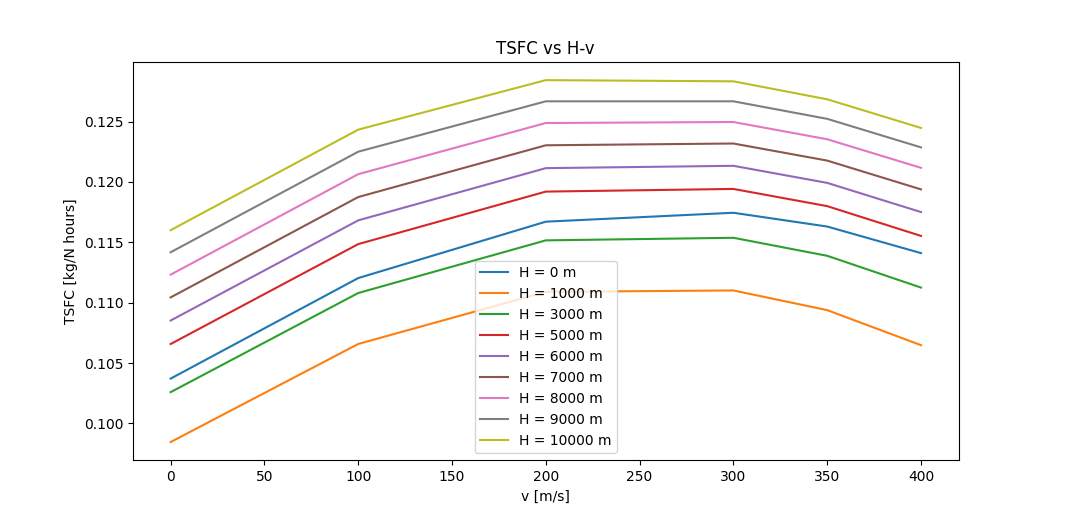
\includegraphics[width=\textwidth]{TSFCHV.png}
  \end{center}

  

  \end{document}